% Options for packages loaded elsewhere
\PassOptionsToPackage{unicode}{hyperref}
\PassOptionsToPackage{hyphens}{url}
%
\documentclass[
]{ctexart}
\usepackage{amsmath,amssymb}
\usepackage{iftex}
\ifPDFTeX
  \usepackage[T1]{fontenc}
  \usepackage[utf8]{inputenc}
  \usepackage{textcomp} % provide euro and other symbols
\else % if luatex or xetex
  \usepackage{unicode-math} % this also loads fontspec
  \defaultfontfeatures{Scale=MatchLowercase}
  \defaultfontfeatures[\rmfamily]{Ligatures=TeX,Scale=1}
\fi
\usepackage{lmodern}
\ifPDFTeX\else
  % xetex/luatex font selection
\fi
% Use upquote if available, for straight quotes in verbatim environments
\IfFileExists{upquote.sty}{\usepackage{upquote}}{}
\IfFileExists{microtype.sty}{% use microtype if available
  \usepackage[]{microtype}
  \UseMicrotypeSet[protrusion]{basicmath} % disable protrusion for tt fonts
}{}
\makeatletter
\@ifundefined{KOMAClassName}{% if non-KOMA class
  \IfFileExists{parskip.sty}{%
    \usepackage{parskip}
  }{% else
    \setlength{\parindent}{0pt}
    \setlength{\parskip}{6pt plus 2pt minus 1pt}}
}{% if KOMA class
  \KOMAoptions{parskip=half}}
\makeatother
\usepackage{xcolor}
\usepackage[margin=2.5cm]{geometry}
\usepackage{color}
\usepackage{fancyvrb}
\newcommand{\VerbBar}{|}
\newcommand{\VERB}{\Verb[commandchars=\\\{\}]}
\DefineVerbatimEnvironment{Highlighting}{Verbatim}{commandchars=\\\{\}}
% Add ',fontsize=\small' for more characters per line
\newenvironment{Shaded}{}{}
\newcommand{\AlertTok}[1]{\textcolor[rgb]{1.00,0.00,0.00}{\textbf{#1}}}
\newcommand{\AnnotationTok}[1]{\textcolor[rgb]{0.38,0.63,0.69}{\textbf{\textit{#1}}}}
\newcommand{\AttributeTok}[1]{\textcolor[rgb]{0.49,0.56,0.16}{#1}}
\newcommand{\BaseNTok}[1]{\textcolor[rgb]{0.25,0.63,0.44}{#1}}
\newcommand{\BuiltInTok}[1]{\textcolor[rgb]{0.00,0.50,0.00}{#1}}
\newcommand{\CharTok}[1]{\textcolor[rgb]{0.25,0.44,0.63}{#1}}
\newcommand{\CommentTok}[1]{\textcolor[rgb]{0.38,0.63,0.69}{\textit{#1}}}
\newcommand{\CommentVarTok}[1]{\textcolor[rgb]{0.38,0.63,0.69}{\textbf{\textit{#1}}}}
\newcommand{\ConstantTok}[1]{\textcolor[rgb]{0.53,0.00,0.00}{#1}}
\newcommand{\ControlFlowTok}[1]{\textcolor[rgb]{0.00,0.44,0.13}{\textbf{#1}}}
\newcommand{\DataTypeTok}[1]{\textcolor[rgb]{0.56,0.13,0.00}{#1}}
\newcommand{\DecValTok}[1]{\textcolor[rgb]{0.25,0.63,0.44}{#1}}
\newcommand{\DocumentationTok}[1]{\textcolor[rgb]{0.73,0.13,0.13}{\textit{#1}}}
\newcommand{\ErrorTok}[1]{\textcolor[rgb]{1.00,0.00,0.00}{\textbf{#1}}}
\newcommand{\ExtensionTok}[1]{#1}
\newcommand{\FloatTok}[1]{\textcolor[rgb]{0.25,0.63,0.44}{#1}}
\newcommand{\FunctionTok}[1]{\textcolor[rgb]{0.02,0.16,0.49}{#1}}
\newcommand{\ImportTok}[1]{\textcolor[rgb]{0.00,0.50,0.00}{\textbf{#1}}}
\newcommand{\InformationTok}[1]{\textcolor[rgb]{0.38,0.63,0.69}{\textbf{\textit{#1}}}}
\newcommand{\KeywordTok}[1]{\textcolor[rgb]{0.00,0.44,0.13}{\textbf{#1}}}
\newcommand{\NormalTok}[1]{#1}
\newcommand{\OperatorTok}[1]{\textcolor[rgb]{0.40,0.40,0.40}{#1}}
\newcommand{\OtherTok}[1]{\textcolor[rgb]{0.00,0.44,0.13}{#1}}
\newcommand{\PreprocessorTok}[1]{\textcolor[rgb]{0.74,0.48,0.00}{#1}}
\newcommand{\RegionMarkerTok}[1]{#1}
\newcommand{\SpecialCharTok}[1]{\textcolor[rgb]{0.25,0.44,0.63}{#1}}
\newcommand{\SpecialStringTok}[1]{\textcolor[rgb]{0.73,0.40,0.53}{#1}}
\newcommand{\StringTok}[1]{\textcolor[rgb]{0.25,0.44,0.63}{#1}}
\newcommand{\VariableTok}[1]{\textcolor[rgb]{0.10,0.09,0.49}{#1}}
\newcommand{\VerbatimStringTok}[1]{\textcolor[rgb]{0.25,0.44,0.63}{#1}}
\newcommand{\WarningTok}[1]{\textcolor[rgb]{0.38,0.63,0.69}{\textbf{\textit{#1}}}}
\usepackage{longtable,booktabs,array}
\usepackage{calc} % for calculating minipage widths
% Correct order of tables after \paragraph or \subparagraph
\usepackage{etoolbox}
\makeatletter
\patchcmd\longtable{\par}{\if@noskipsec\mbox{}\fi\par}{}{}
\makeatother
% Allow footnotes in longtable head/foot
\IfFileExists{footnotehyper.sty}{\usepackage{footnotehyper}}{\usepackage{footnote}}
\makesavenoteenv{longtable}
\usepackage{graphicx}
\makeatletter
\def\maxwidth{\ifdim\Gin@nat@width>\linewidth\linewidth\else\Gin@nat@width\fi}
\def\maxheight{\ifdim\Gin@nat@height>\textheight\textheight\else\Gin@nat@height\fi}
\makeatother
% Scale images if necessary, so that they will not overflow the page
% margins by default, and it is still possible to overwrite the defaults
% using explicit options in \includegraphics[width, height, ...]{}
\setkeys{Gin}{width=\maxwidth,height=\maxheight,keepaspectratio}
% Set default figure placement to htbp
\makeatletter
\def\fps@figure{htbp}
\makeatother
\setlength{\emergencystretch}{3em} % prevent overfull lines
\providecommand{\tightlist}{%
  \setlength{\itemsep}{0pt}\setlength{\parskip}{0pt}}
\setcounter{secnumdepth}{-\maxdimen} % remove section numbering
\ifLuaTeX
  \usepackage{selnolig}  % disable illegal ligatures
\fi
\IfFileExists{bookmark.sty}{\usepackage{bookmark}}{\usepackage{hyperref}}
\IfFileExists{xurl.sty}{\usepackage{xurl}}{} % add URL line breaks if available
\urlstyle{same}
\hypersetup{
  pdftitle={胸部 X 光肺炎识别模型的构建、评价与跨数据集泛化分析},
  hidelinks,
  pdfcreator={LaTeX via pandoc}}

\title{胸部 X 光肺炎识别模型的构建、评价与跨数据集泛化分析}
\usepackage{etoolbox}
\makeatletter
\providecommand{\subtitle}[1]{% add subtitle to \maketitle
  \apptocmd{\@title}{\par {\large #1 \par}}{}{}
}
\makeatother
\subtitle{《模式识别与机器学习》课程设计}
\author{}
\date{}

\begin{document}
\maketitle

\hypertarget{ux6458-ux8981}{%
\subsection{摘 要}\label{ux6458-ux8981}}

胸部 X 光图像常用于肺炎的辅助判断。本课程设计围绕``肺炎 X
光图像诊断识别''题目，完成了一个正常/肺炎二分类实验，内容包括数据检查、图像预处理、模型训练、测试评价、误差分析和网页演示。实验使用
Chest X-Ray Images (Pneumonia) 数据集。本地逐文件检查后，共得到 5856
张可读取图像，其中训练集 5216 张、验证集 16 张、测试集 624 张。

实验比较了 EfficientNetV2-S 和 Vision Transformer
两类模型。输入图像统一缩放到 224 × 224，并按 ImageNet
均值和标准差归一化；训练时加入随机水平翻转和小角度旋转。模型输出正常类和肺炎类概率，默认分类阈值设为
0.5。训练使用交叉熵损失和 AdamW 优化器，部分类别不均衡实验加入类别权重。

在默认阈值下，ImageNet 预训练 ViT-B/16
是本组实验中综合表现较好的模型，测试集 accuracy 为 0.9006，precision 为
0.8779，recall 为 0.9769，specificity 为 0.7735，F1 为 0.9248，ROC-AUC
为 0.9710。与 EfficientNetV2-S 无类别权重实验相比，ViT-B/16
将正常样本误报数从 91 降至 53，同时保持较高的肺炎召回率。原始
EfficientNetV2-S 在测试集阈值扫描中达到最高 F1
0.9527，但该阈值直接来自测试集预测结果，只适合做阈值权衡分析，不能作为无偏部署阈值。独立校准集实验显示，从训练集中划出的校准阈值没有稳定迁移到官方测试集，因此最终结论仍采用默认阈值结果。

Grad-CAM
结果显示，卷积模型在部分样本上会关注胸腔内部区域，但热力图只能辅助理解模型行为，不能当作医学病灶定位证据。课程设计还实现了单图上传网页演示，用于展示从上传胸片到输出分类概率的过程。综合默认阈值、误差结构和阈值分析，预训练
ViT-B/16 更适合作为本报告的主模型，EfficientNetV2-S
的测试集阈值扫描结果作为补充分析。实验结果只用于课程设计和研究训练，不构成临床诊断依据。

\textbf{关键词}：胸部 X 光；肺炎识别；二分类；EfficientNetV2；Vision
Transformer；迁移学习

\hypertarget{abstract}{%
\subsection{Abstract}\label{abstract}}

Chest X-ray images are widely used as auxiliary evidence for pneumonia
assessment. This course-design project builds a normal-versus-pneumonia
classification experiment, covering data checking, preprocessing, model
training, test evaluation, error analysis, and a local web
demonstration. After local file-level checking, the Chest X-Ray Images
(Pneumonia) dataset contains 5,856 readable images, including 5,216
training images, 16 validation images, and 624 test images.

Two model families are compared: EfficientNetV2-S and Vision
Transformer. Images are resized to 224 × 224, normalized using ImageNet
statistics, and augmented during training by random horizontal flipping
and small-angle rotation. The classifier predicts probabilities for the
normal and pneumonia classes, and the default decision threshold is 0.5.
Cross-entropy loss and AdamW optimization are used, with class weights
tested in part of the experiments.

Among the compared models, the ImageNet-pretrained ViT-B/16 gives the
strongest default-threshold result, with accuracy 0.9006, precision
0.8779, recall 0.9769, specificity 0.7735, F1 0.9248, and ROC-AUC 0.9710
on the test set. The original EfficientNetV2-S baseline reaches a higher
threshold-swept F1 of 0.9527, but this threshold is selected from
test-set predictions and is used only for trade-off analysis. Grad-CAM
is used for qualitative interpretation of the CNN baseline, and a local
web demo shows the single-image upload and prediction process. The
experiment is limited to a pattern-recognition course project and is not
a clinical diagnostic system.

\textbf{Keywords}: chest X-ray; pneumonia recognition; binary
classification; EfficientNetV2; Vision Transformer; transfer learning

\hypertarget{ux5f15ux8a00}{%
\subsection{1 引言}\label{ux5f15ux8a00}}

肺炎是常见的呼吸系统疾病。胸部 X
光图像能够反映肺部阴影、纹理改变和局部浸润等影像特征，因此常被用于肺炎诊断的辅助判断。传统模式识别方法通常依赖人工设计纹理、边缘或灰度统计特征，而深度学习模型可以直接从图像中学习多层次视觉特征，在医学图像分类中已经成为常用技术路线之一
{[}3{]}。

本课程设计的任务是根据胸部 X
光图像判断样本属于正常类还是肺炎类。该问题可以形式化为二分类任务：输入一张胸片图像，输出两个类别的概率，再根据阈值给出最终类别。工作范围限定在课程设计实验，不面向临床诊断。

具体工作包括四部分：检查数据集文件和类别分布；训练并比较
EfficientNetV2-S 与 ViT-B/16；用混淆矩阵、误差率、概率分布、阈值扫描和
Grad-CAM
分析模型表现；最后把选定模型接入本地网页，展示单张胸片上传后的推理结果。已有研究已经将卷积网络和
Transformer 用于胸片肺炎检测 {[}4,
8{]}，本报告重点放在课程设计要求下的复现、比较和边界分析。

\hypertarget{ux6570ux636eux96c6ux4e0eux9884ux5904ux7406}{%
\subsection{2
数据集与预处理}\label{ux6570ux636eux96c6ux4e0eux9884ux5904ux7406}}

\hypertarget{ux6570ux636eux96c6ux7ec4ux6210}{%
\subsubsection{2.1 数据集组成}\label{ux6570ux636eux96c6ux7ec4ux6210}}

实验使用 Chest X-Ray Images (Pneumonia) 数据集。该数据集来自 Kermany
等发布的儿童胸部 X 光图像数据 {[}1,
2{]}。原始目录已经划分为训练集、验证集和测试集，并按正常类与肺炎类存放。文件夹名对应图像标签，可直接生成二分类标签。课程资料和公开页面中常见的总数表述为
5863；本地逐文件读取后，有 5856
张图像可以正常参与实验。后续统计和实验均以这一本地可读数量为准。样本数量如表
1 所示。

\begin{longtable}[]{@{}lrrr@{}}
\caption{数据集样本数量统计}\tabularnewline
\toprule\noalign{}
数据划分 & 正常类 & 肺炎类 & 合计 \\
\midrule\noalign{}
\endfirsthead
\toprule\noalign{}
数据划分 & 正常类 & 肺炎类 & 合计 \\
\midrule\noalign{}
\endhead
\bottomrule\noalign{}
\endlastfoot
训练集 & 1341 & 3875 & 5216 \\
验证集 & 8 & 8 & 16 \\
测试集 & 234 & 390 & 624 \\
总计 & 1583 & 4273 & 5856 \\
\end{longtable}

训练集中肺炎样本占 74.3\%，正常样本占 25.7\%，肺炎与正常样本数约为
2.89:1；测试集中肺炎样本占 62.5\%，肺炎与正常样本数约为
1.67:1。训练集比测试集更偏向肺炎类别，模型可能因此更倾向于把样本判为肺炎。验证集只有
16 张图像，虽然正常类和肺炎类各 8
张，但样本量过小，不适合承担稳定的模型选择或阈值校准功能。因此，模型比较主要依据测试集结果，同时在结论中保留这一限制。

\hypertarget{ux56feux50cfux9884ux5904ux7406}{%
\subsubsection{2.2 图像预处理}\label{ux56feux50cfux9884ux5904ux7406}}

模型不能直接处理原始图像文件。实验中先将图像读取为三通道格式，再统一调整为
224 × 224 大小，并使用 ImageNet
的均值和标准差进行归一化。训练阶段加入随机水平翻转和小角度旋转，以增加样本变化；验证和测试阶段不使用随机增强，保证评估结果稳定。

这样处理后，每张胸片都被转换成固定尺寸的数值张量。模型实际学习的是图像中亮度、边缘、纹理、阴影分布和整体结构对应的数值模式。

\hypertarget{ux65b9ux6cd5}{%
\subsection{3 方法}\label{ux65b9ux6cd5}}

\hypertarget{ux4e8cux5206ux7c7bux57faux672cux539fux7406}{%
\subsubsection{3.1
二分类基本原理}\label{ux4e8cux5206ux7c7bux57faux672cux539fux7406}}

肺炎识别在本实验中被建模为二分类概率预测。对一张输入图像，模型输出正常类和肺炎类两个分数，再通过
softmax 转换为概率。默认判别规则为：若肺炎类概率满足
\(P(\mathrm{pneumonia}) \ge 0.5\)，则预测为肺炎；否则预测为正常。

训练时，每张图像都有真实标签。如果真实标签为肺炎而模型给出的肺炎概率较低，交叉熵损失会变大；如果真实标签为正常而模型给出的肺炎概率过高，损失同样会变大。优化器根据损失函数对模型参数进行更新，使模型逐渐提高正确类别的概率，降低错误类别的概率。

模型没有采用人工规则去判断``哪里有阴影''。训练过程利用带标签胸片学习两类图像在统计特征上的差异，训练完成后形成从图像到类别概率的映射。

\hypertarget{efficientnetv2-s-ux6a21ux578b}{%
\subsubsection{3.2 EfficientNetV2-S
模型}\label{efficientnetv2-s-ux6a21ux578b}}

EfficientNetV2-S
属于卷积神经网络。卷积网络的特点是从局部区域开始提取特征：浅层更容易学习边缘、纹理和亮暗变化，深层会逐渐组合出更复杂的胸部结构和异常影像模式。实验使用
ImageNet 预训练的
EfficientNetV2-S，并将最后的分类层改为正常类和肺炎类两个输出。

选择 EfficientNetV2-S
的原因有两点。一是它在图像分类任务中具有较好的精度和计算效率平衡；二是卷积网络可以配合
Grad-CAM 进行可解释性可视化，便于观察模型在胸片上的大致关注区域。

\hypertarget{vision-transformer-ux6a21ux578b}{%
\subsubsection{3.3 Vision Transformer
模型}\label{vision-transformer-ux6a21ux578b}}

Vision Transformer
与卷积网络不同。它先将图像切分为若干小块，再将每个图像块转换为
token，通过 self-attention 建立不同区域之间的关系。以 ViT-B/16
为例，图像被划分为 16 × 16
的小块，模型可以同时参考左右肺野、上肺和下肺、肺部边缘以及整体胸腔结构。

Transformer
更擅长建模较长距离的区域关系，但从零训练通常需要更多数据。本任务数据规模有限，因此采用
ImageNet 预训练 ViT-B/16 进行微调。后续结果也显示，预训练对 ViT
路线影响很大。

\hypertarget{ux8badux7ec3ux4e0eux8bc4ux4ef7ux6307ux6807}{%
\subsubsection{3.4
训练与评价指标}\label{ux8badux7ec3ux4e0eux8bc4ux4ef7ux6307ux6807}}

EfficientNetV2-S 是 EfficientNet
系列的改进版本，设计目标是在精度、参数效率和训练速度之间取得更好的平衡
{[}5{]}。原始 EfficientNetV2-S 基线使用 ImageNet 预训练权重训练 3 个
epoch，batch size 为 32，初始学习率为 0.0003。ViT-B/16 采用 torchvision
提供的 ImageNet-1K 预训练权重训练 4 个 epoch，batch size 为
16，初始学习率为 0.00005。两类模型均使用 AdamW 优化器、余弦学习率调度和
0.0001 权重衰减，随机种子固定为
42。部分类别不均衡实验加入类别权重，未加权实验则使用普通交叉熵损失。

测试集共有 624 张图像，其中正常类 234 张，肺炎类 390
张。评价指标包括准确率、精确率、召回率、特异性、F1、ROC-AUC
和混淆矩阵。其中召回率反映肺炎样本被识别出来的比例，特异性反映正常样本被正确排除的比例。设
TP、TN、FP、FN 分别表示真阳性、真阴性、假阳性和假阴性，则 accuracy = (TP
+ TN) / (TP + TN + FP + FN)，precision = TP / (TP + FP)，recall = TP /
(TP + FN)，specificity = TN / (TN + FP)，F1 = 2 × precision × recall /
(precision + recall)。

医学图像分类不能只看单一指标。例如，模型更倾向于预测肺炎时，召回率可能提高，但正常样本误报也会增加。因此，报告同时观察召回率、特异性、混淆矩阵、假阳性率、假阴性率、平衡准确率和模型输出概率分布。新增的二次统计均由已保存预测结果和评估结果计算得到，不重新训练模型。

\hypertarget{ux5b9eux9a8cux7ed3ux679cux4e0eux5206ux6790}{%
\subsection{4
实验结果与分析}\label{ux5b9eux9a8cux7ed3ux679cux4e0eux5206ux6790}}

\hypertarget{ux9ed8ux8ba4ux9608ux503cux7ed3ux679c}{%
\subsubsection{4.1
默认阈值结果}\label{ux9ed8ux8ba4ux9608ux503cux7ed3ux679c}}

表 2 给出了默认阈值 0.5 下各模型在测试集上的结果。

\begin{longtable}[]{@{}lrrrrrr@{}}
\caption{默认阈值下不同模型测试集结果}\tabularnewline
\toprule\noalign{}
模型 & Acc & Prec & Rec & Spec & F1 & AUC \\
\midrule\noalign{}
\endfirsthead
\toprule\noalign{}
模型 & Acc & Prec & Rec & Spec & F1 & AUC \\
\midrule\noalign{}
\endhead
\bottomrule\noalign{}
\endlastfoot
E-V2 原始 & 0.8173 & 0.7760 & 0.9949 & 0.5214 & 0.8719 & 0.9780 \\
E-V2 无权重 & 0.8510 & 0.8100 & 0.9949 & 0.6111 & 0.8930 & 0.9626 \\
ViT-S 随机 & 0.7949 & 0.7937 & 0.9077 & 0.6068 & 0.8469 & 0.8748 \\
ViT-B 加权 & 0.9006 & 0.8779 & 0.9769 & 0.7735 & 0.9248 & 0.9710 \\
ViT-B 无权重 & 0.8862 & 0.8537 & 0.9872 & 0.7179 & 0.9156 & 0.9676 \\
\end{longtable}

表中 Acc、Prec、Rec、Spec 和 AUC
分别表示准确率、精确率、召回率、特异性和 ROC-AUC；E-V2 表示
EfficientNetV2-S。``加权''表示训练时加入类别权重，``无权重''表示使用普通交叉熵损失。ViT-S
随机表示没有成功加载外部预训练权重的 ViT-Small
对照实验。在这些模型中，预训练 ViT-B/16
加类别权重的默认阈值结果最好。它在测试集中正确识别 181 张正常图像和 381
张肺炎图像，误报 53 张正常图像，漏检 9 张肺炎图像。与 EfficientNetV2-S
无权重实验相比，ViT-B/16 的 F1 从 0.8930 提高到 0.9248，特异性从 0.6111
提高到 0.7735，正常样本误报明显减少。

\begin{figure}
\centering
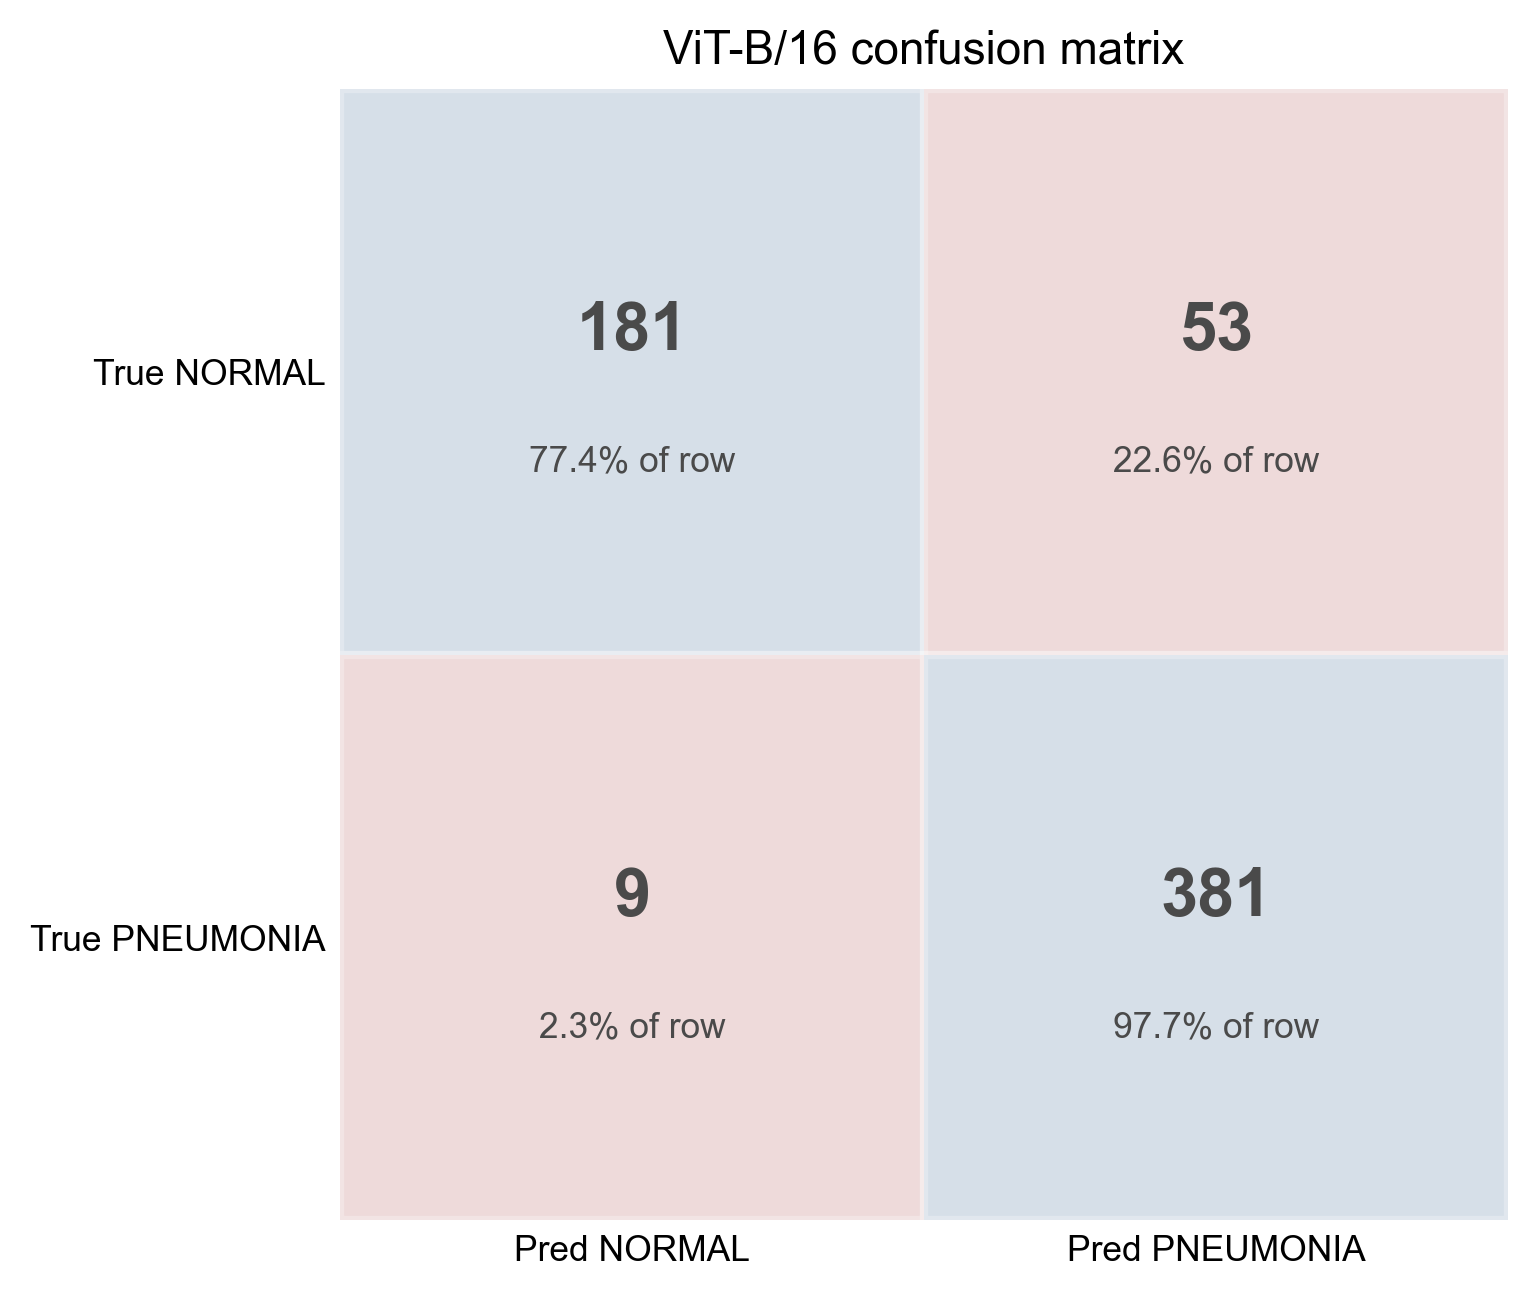
\includegraphics{../figures/confusion_matrix_test_vit_b16.png}
\caption{ViT-B/16 测试集混淆矩阵}
\end{figure}

\hypertarget{ux9ed8ux8ba4ux9608ux503cux8befux5deeux7ed3ux6784ux4e0eux6982ux7387ux5206ux5e03}{%
\subsubsection{4.2
默认阈值误差结构与概率分布}\label{ux9ed8ux8ba4ux9608ux503cux8befux5deeux7ed3ux6784ux4e0eux6982ux7387ux5206ux5e03}}

默认阈值下，ViT-B/16 的主要优势在于减少正常样本误报。表 3
将混淆矩阵转换为假阳性率、假阴性率、平衡准确率和阴性预测值。假阳性率表示正常图像被误判为肺炎的比例，假阴性率表示肺炎图像被漏检的比例，平衡准确率可以减轻类别不均衡对
accuracy 的影响。

\begin{longtable}[]{@{}lrrrrrrrr@{}}
\caption{默认阈值下的错误结构分析}\tabularnewline
\toprule\noalign{}
模型 & TN & FP & FN & TP & FPR & FNR & Bal-Acc & NPV \\
\midrule\noalign{}
\endfirsthead
\toprule\noalign{}
模型 & TN & FP & FN & TP & FPR & FNR & Bal-Acc & NPV \\
\midrule\noalign{}
\endhead
\bottomrule\noalign{}
\endlastfoot
E-V2 原始 & 122 & 112 & 2 & 388 & 47.9\% & 0.5\% & 0.7581 & 0.9839 \\
E-V2 无权重 & 143 & 91 & 2 & 388 & 38.9\% & 0.5\% & 0.8030 & 0.9862 \\
ViT-S 随机 & 142 & 92 & 36 & 354 & 39.3\% & 9.2\% & 0.7573 & 0.7978 \\
ViT-B 加权 & 181 & 53 & 9 & 381 & 22.6\% & 2.3\% & 0.8752 & 0.9526 \\
ViT-B 无权重 & 168 & 66 & 5 & 385 & 28.2\% & 1.3\% & 0.8526 & 0.9711 \\
\end{longtable}

EfficientNetV2-S
两个主要实验的假阴性率都很低，但正常样本误报率较高。E-V2
无权重实验的假阳性率为 38.9\%，也就是 234 张正常测试图像中有 91
张被判为肺炎。ViT-B/16 加权模型的假阳性率为 22.6\%，假阴性率为
2.3\%。相较之下，它在正常误报和肺炎漏检之间更均衡。

\begin{figure}
\centering
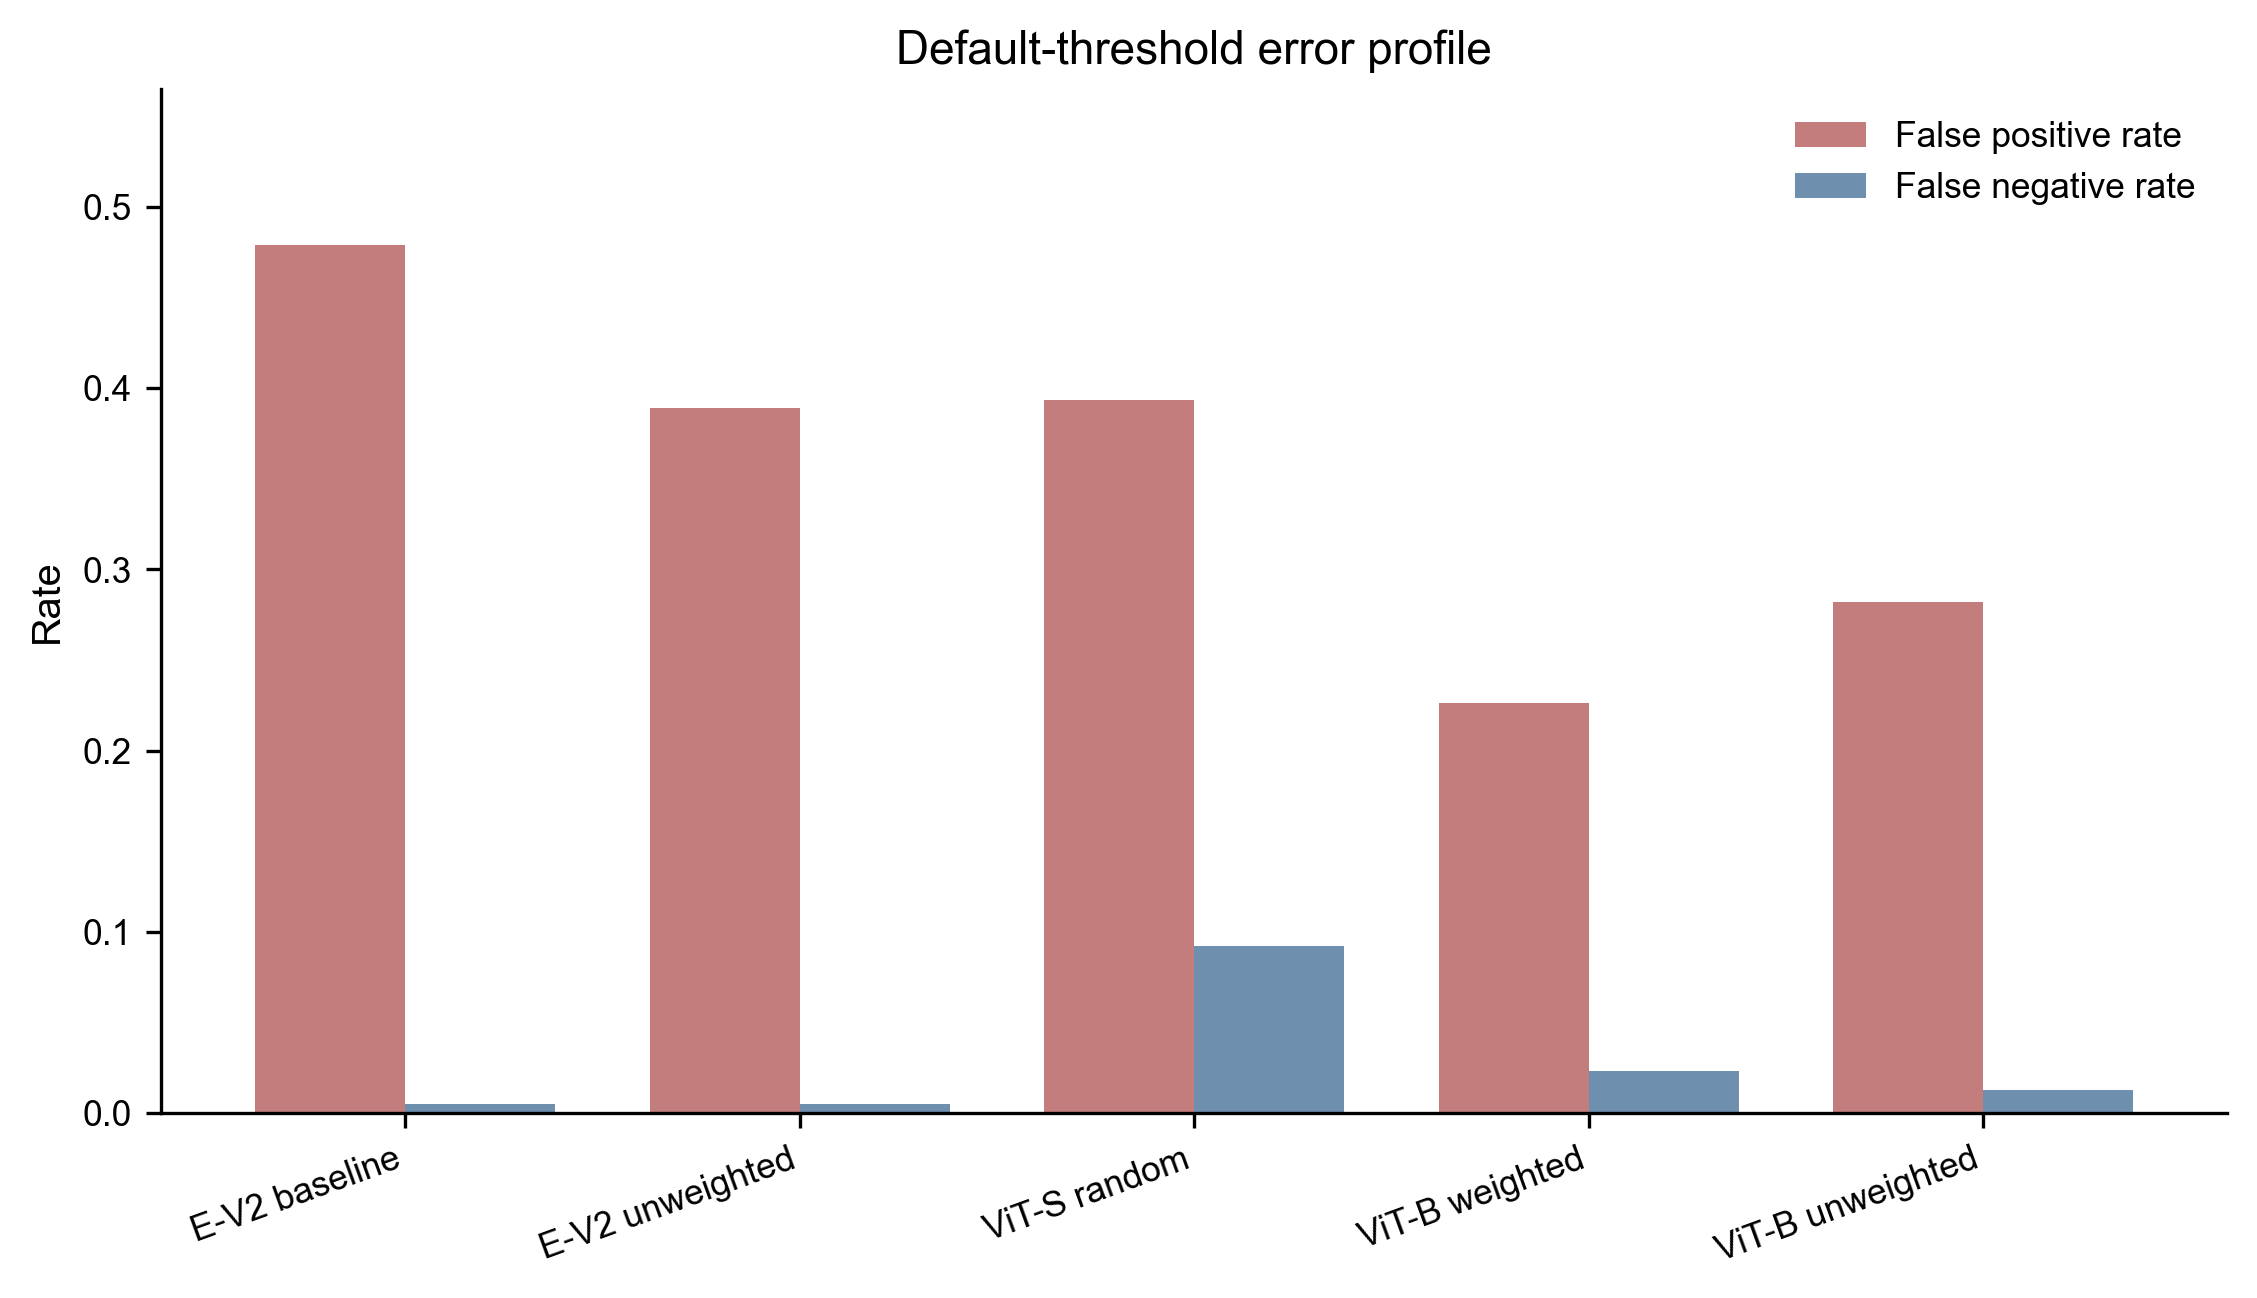
\includegraphics[width=1\textwidth,height=\textheight]{../figures/error_profile_default_threshold.png}
\caption{默认阈值误差率对比}
\end{figure}

按文件名中的肺炎类型继续统计，测试集肺炎图像包括 242 张细菌性肺炎和 148
张病毒性肺炎。ViT-B/16 加权模型在细菌性肺炎子集上识别出 238/242 张，漏检
4 张；在病毒性肺炎子集上识别出 143/148 张，漏检 5 张。随机初始化
ViT-Small
在两个肺炎子集上的漏检数更多，说明预训练对肺炎样本内部的识别稳定性也有帮助。表中的``148/148''只表示该测试子集没有漏检，不能说明模型在更大人群或新数据上也不会漏检。

\begin{longtable}[]{@{}lrrrr@{}}
\caption{测试集肺炎子类型召回率}\tabularnewline
\toprule\noalign{}
模型 & 细菌性识别/总数 & 细菌性漏检 & 病毒性识别/总数 & 病毒性漏检 \\
\midrule\noalign{}
\endfirsthead
\toprule\noalign{}
模型 & 细菌性识别/总数 & 细菌性漏检 & 病毒性识别/总数 & 病毒性漏检 \\
\midrule\noalign{}
\endhead
\bottomrule\noalign{}
\endlastfoot
E-V2 原始 & 240/242 & 2 & 148/148 & 0 \\
E-V2 无权重 & 241/242 & 1 & 147/148 & 1 \\
ViT-S 随机 & 218/242 & 24 & 136/148 & 12 \\
ViT-B 加权 & 238/242 & 4 & 143/148 & 5 \\
ViT-B 无权重 & 239/242 & 3 & 146/148 & 2 \\
\end{longtable}

模型输出概率可以帮助定位部分错误来源。对 ViT-B/16
加权模型，真实正常样本的肺炎概率中位数为
0.0368，说明多数正常图像被赋予较低肺炎概率；但正常样本的第 90
百分位数达到
0.9691，说明仍有一部分正常图像被高置信度推向肺炎类。真实肺炎样本的肺炎概率中位数为
0.9996，大多数肺炎图像被明显区分出来。所有错误样本共 62 张，其中 35
张错误样本的预测置信度不低于
0.9。这类错误既包括阈值附近的摇摆样本，也包括高置信误判。

\begin{longtable}[]{@{}lrrrrrr@{}}
\caption{ViT-B/16 加权模型输出肺炎概率分布}\tabularnewline
\toprule\noalign{}
真实类别 & 样本数 & 肺炎概率均值 & P10 & P50 & P90 & 0.4--0.6 样本数 \\
\midrule\noalign{}
\endfirsthead
\toprule\noalign{}
真实类别 & 样本数 & 肺炎概率均值 & P10 & P50 & P90 & 0.4--0.6 样本数 \\
\midrule\noalign{}
\endhead
\bottomrule\noalign{}
\endlastfoot
NORMAL & 234 & 0.2588 & 0.0019 & 0.0368 & 0.9691 & 8 \\
PNEUMONIA & 390 & 0.9702 & 0.9810 & 0.9996 & 0.9999 & 3 \\
\end{longtable}

\begin{figure}
\centering
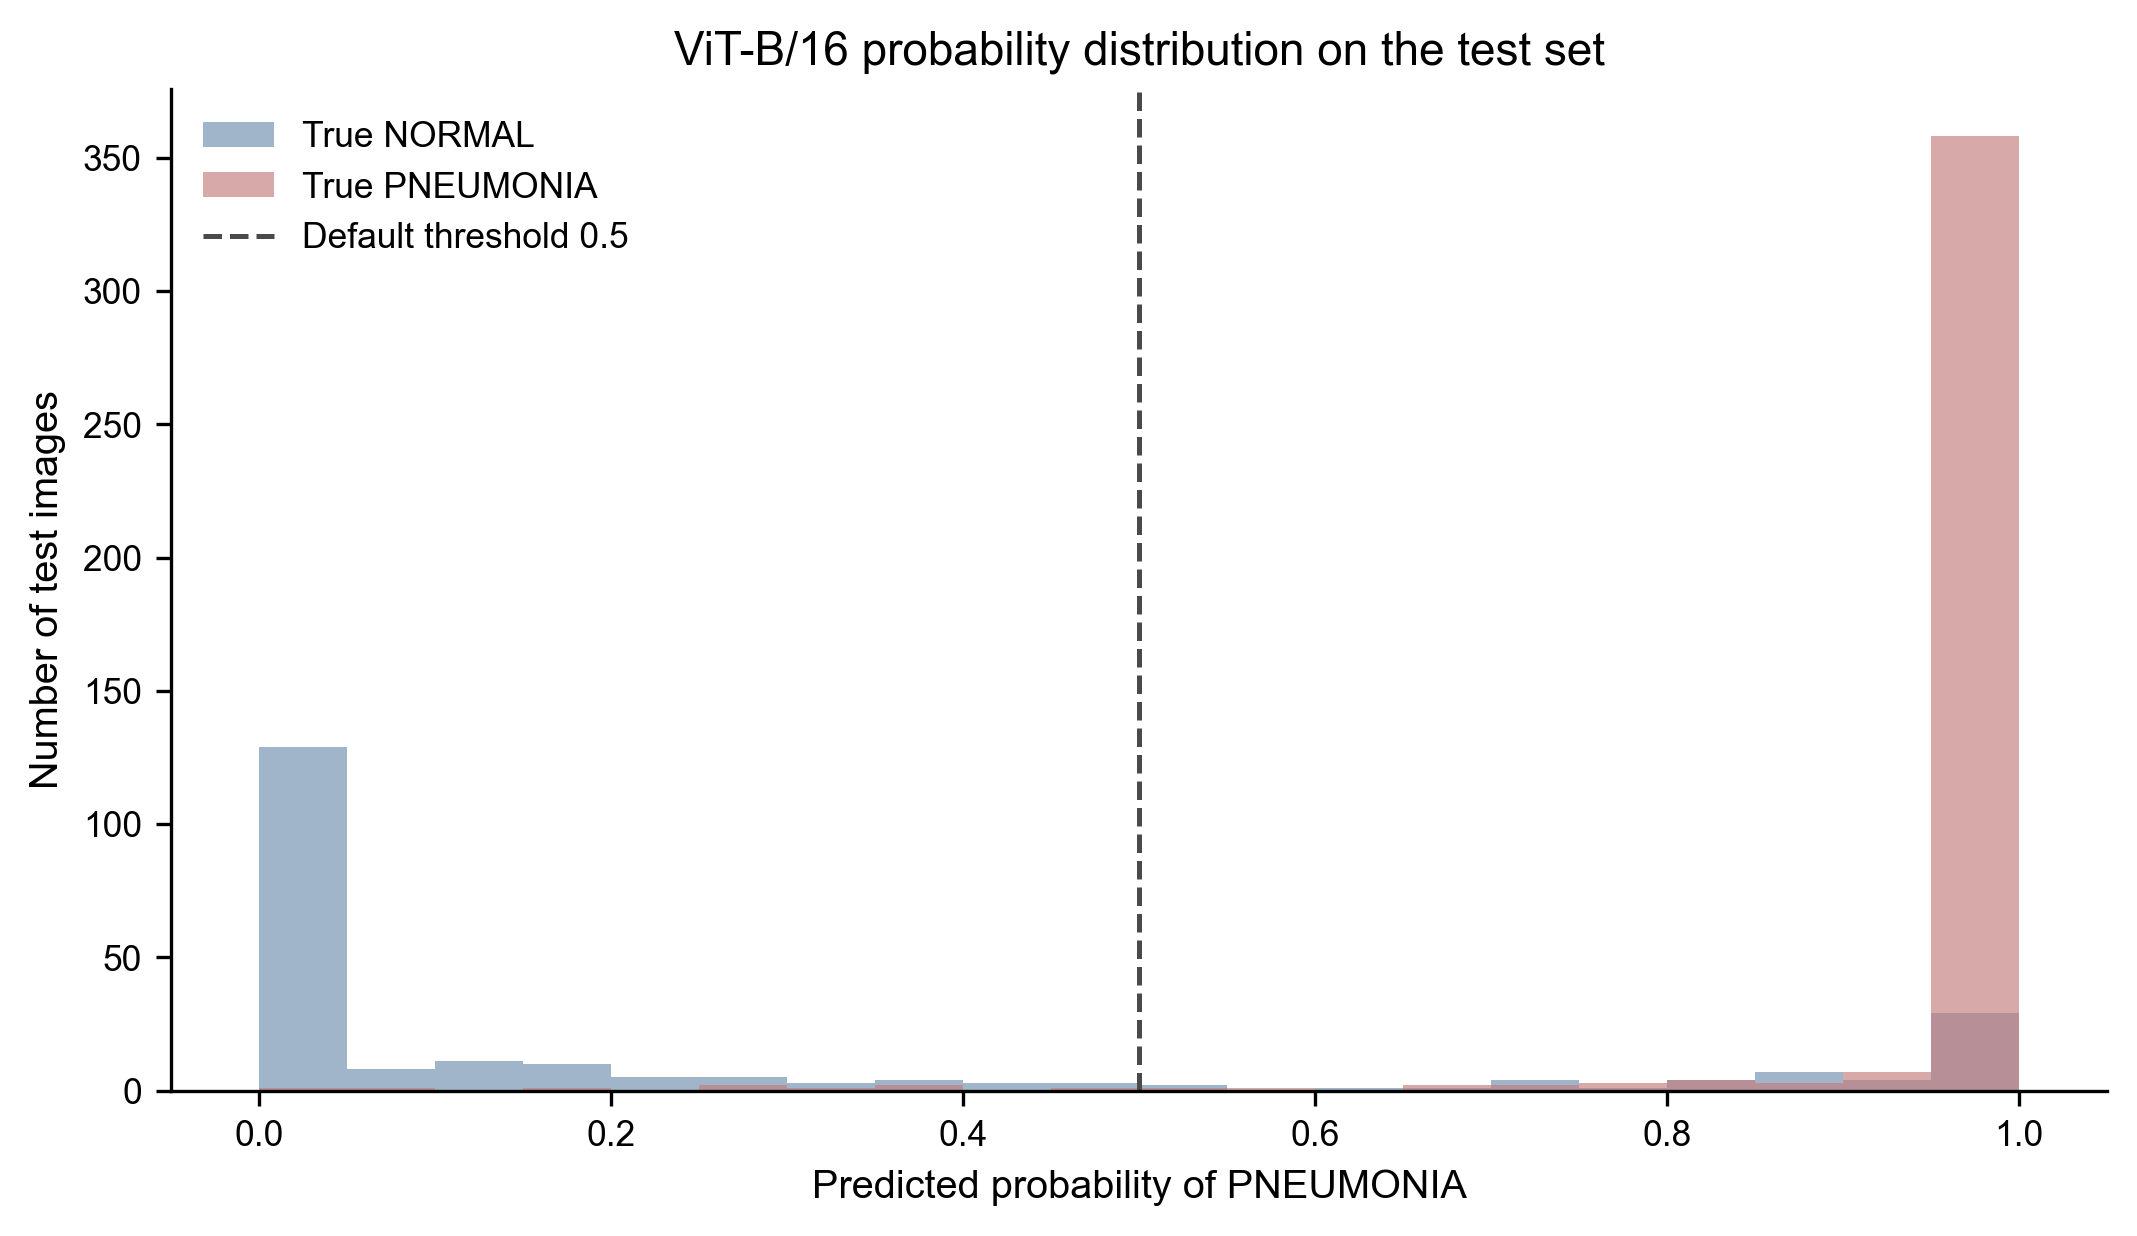
\includegraphics[width=1\textwidth,height=\textheight]{../figures/probability_distribution_test_vit_b16.png}
\caption{ViT-B/16 测试集肺炎概率分布}
\end{figure}

\hypertarget{ux9608ux503cux5206ux6790}{%
\subsubsection{4.3 阈值分析}\label{ux9608ux503cux5206ux6790}}

默认阈值不一定是最合适的操作点。降低阈值会让模型更容易判为肺炎，通常可以提高
recall，但正常样本误报会增加；提高阈值可能提高
specificity，但肺炎漏检也会增加。因此，报告扫描了不同肺炎概率阈值，用来观察模型分数的可调节空间。

\begin{longtable}[]{@{}lrrrrrr@{}}
\caption{测试集阈值扫描结果}\tabularnewline
\toprule\noalign{}
模型 & 阈值 & Acc & Prec & Rec & Spec & F1 \\
\midrule\noalign{}
\endfirsthead
\toprule\noalign{}
模型 & 阈值 & Acc & Prec & Rec & Spec & F1 \\
\midrule\noalign{}
\endhead
\bottomrule\noalign{}
\endlastfoot
E-V2 原始 & 0.997 & 0.9407 & 0.9491 & 0.9564 & 0.9145 & 0.9527 \\
E-V2 无权重 & 0.987 & 0.9135 & 0.9221 & 0.9410 & 0.8675 & 0.9315 \\
ViT-B 加权 & 0.889 & 0.9087 & 0.9132 & 0.9436 & 0.8504 & 0.9281 \\
ViT-B 无权重 & 0.686 & 0.9006 & 0.8779 & 0.9769 & 0.7735 & 0.9248 \\
\end{longtable}

阈值扫描后，原始 EfficientNetV2-S 的测试集 F1 最高，达到 0.9527。预训练
ViT-B/16 在默认阈值下表现更好，但在同一测试集阈值扫描条件下没有超过
EfficientNetV2-S。两条路线的优势并不完全相同：ViT-B/16
适合作为默认阈值分类器，EfficientNetV2-S
的分数排序能力在该测试集上仍有较高上限。

以 ViT-B/16 加权模型为例，如果希望测试集召回率不低于 0.99，阈值需要降到
0.267，此时漏检降为 3 张，但误报增至 69 张；如果接受召回率约
0.95，阈值可升到 0.808，误报降为 41 张，但漏检增至 18
张。阈值选择本质上是在误报和漏检之间取舍，不能只追求某一个数值最大。

\begin{longtable}[]{@{}lrrrrrr@{}}
\caption{ViT-B/16 加权模型测试集阈值操作点}\tabularnewline
\toprule\noalign{}
操作点 & 阈值 & FP & FN & Rec & Spec & F1 \\
\midrule\noalign{}
\endfirsthead
\toprule\noalign{}
操作点 & 阈值 & FP & FN & Rec & Spec & F1 \\
\midrule\noalign{}
\endhead
\bottomrule\noalign{}
\endlastfoot
recall\textgreater=0.990 & 0.267 & 69 & 3 & 0.9923 & 0.7051 & 0.9149 \\
recall\textgreater=0.980 & 0.387 & 59 & 7 & 0.9821 & 0.7479 & 0.9207 \\
recall\textgreater=0.950 & 0.808 & 41 & 18 & 0.9538 & 0.8248 & 0.9265 \\
test best F1 & 0.889 & 35 & 22 & 0.9436 & 0.8504 & 0.9281 \\
\end{longtable}

上述阈值均来自测试集预测结果扫描，只能用于分析精确率、召回率和特异性之间的权衡，不能作为实际使用阈值。若要确定固定阈值，应先划分独立校准集，在校准集上选定阈值，再只用测试集做一次最终评价。

\begin{figure}
\centering
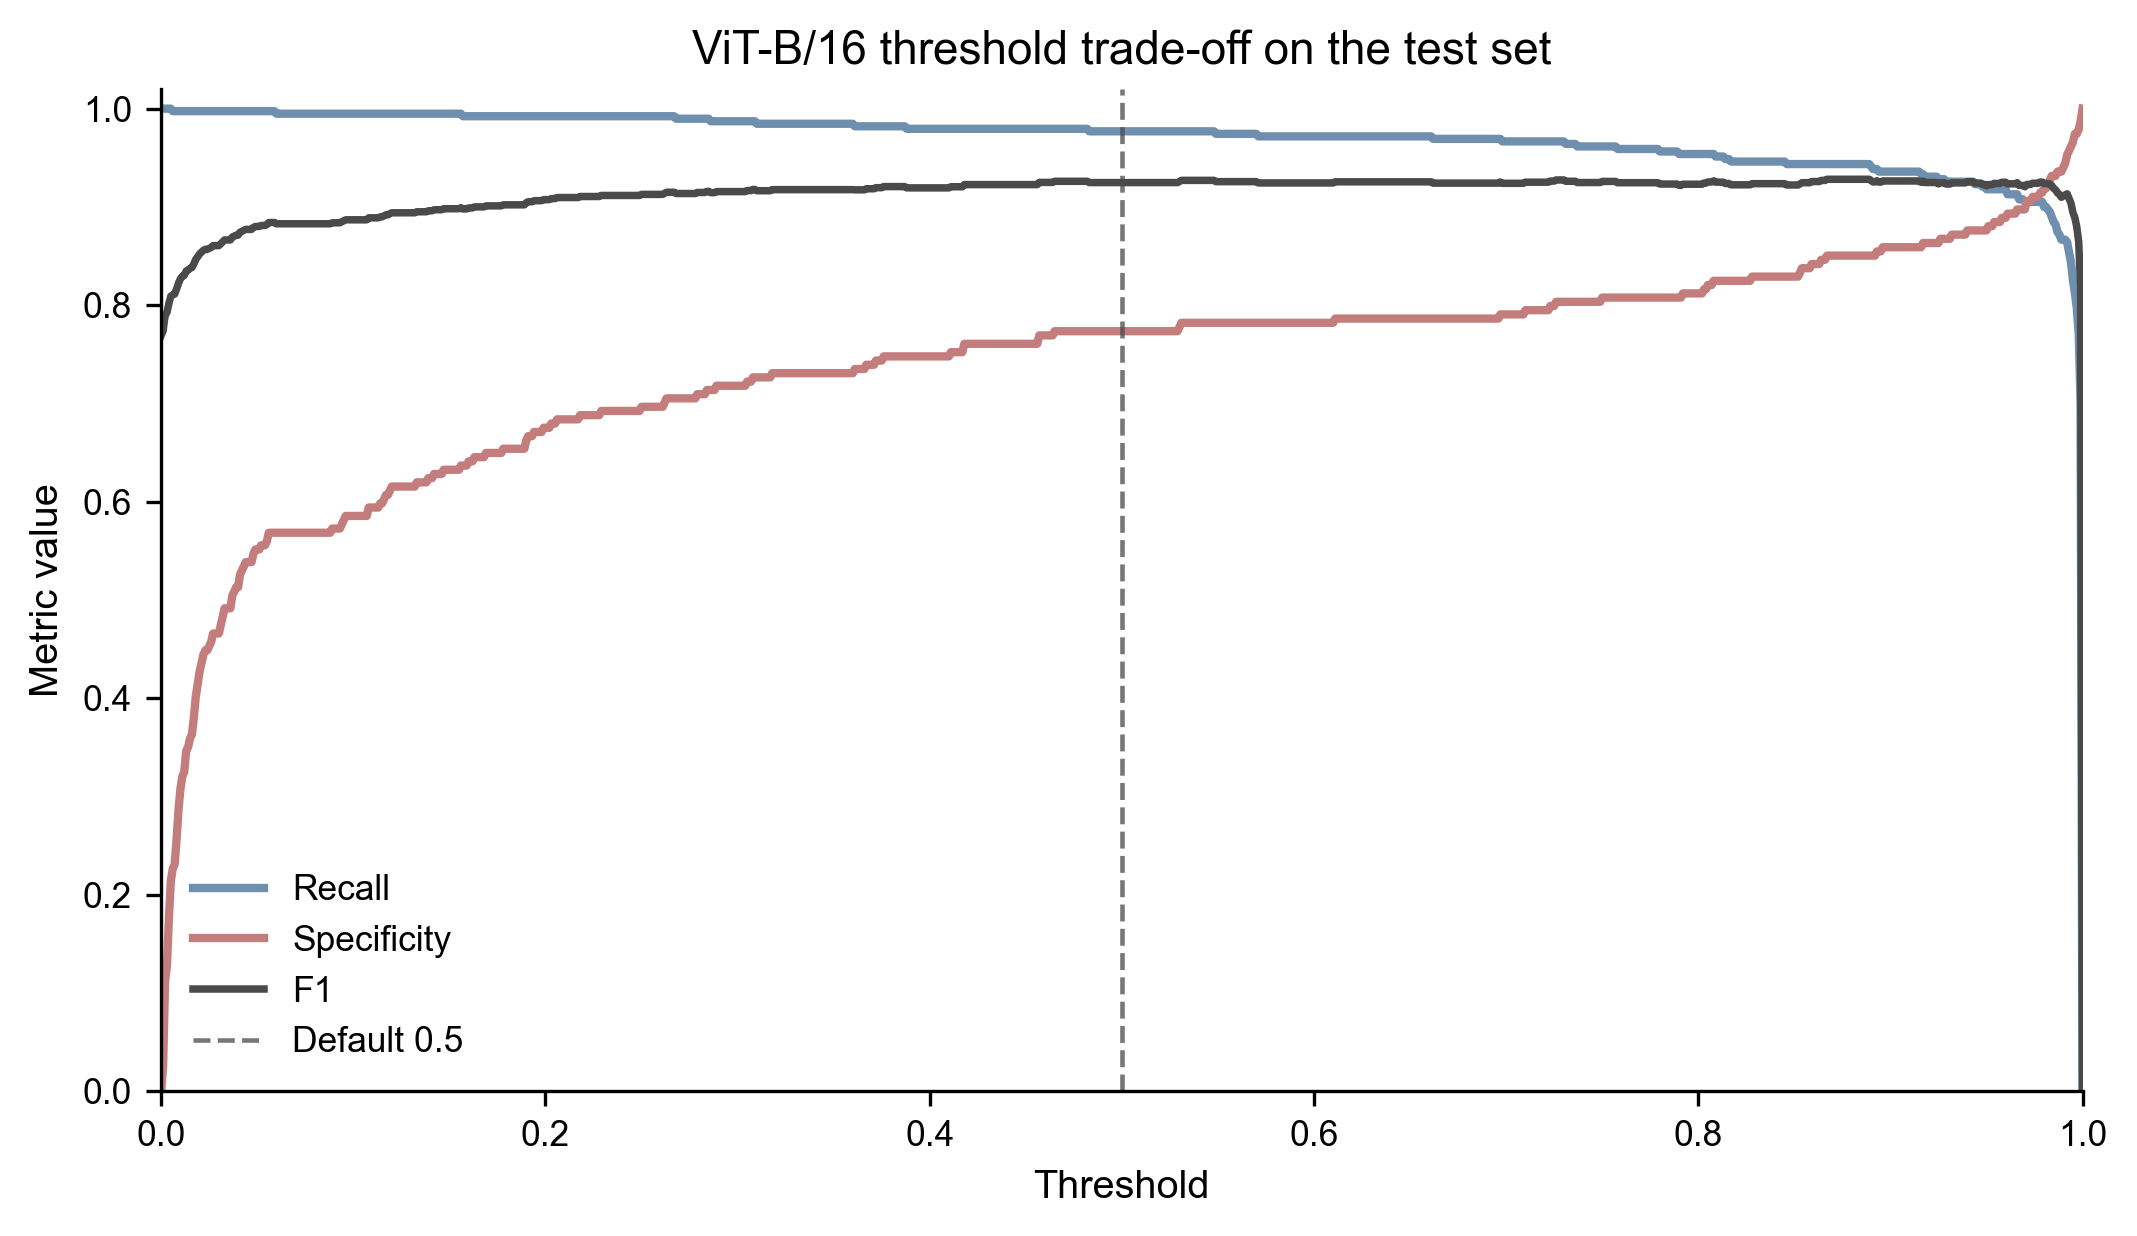
\includegraphics{../figures/threshold_curve_test_vit_b16.png}
\caption{ViT-B/16 测试集阈值曲线}
\end{figure}

\hypertarget{ux72ecux7acbux6821ux51c6ux96c6ux5c1dux8bd5}{%
\subsubsection{4.4
独立校准集尝试}\label{ux72ecux7acbux6821ux51c6ux96c6ux5c1dux8bd5}}

为了检验训练集内部校准阈值是否能带来稳定提升，实验又从训练集中划出 10\%
图像作为校准集，并用剩余训练图像重新训练
ViT-B/16。校准集没有参与该模型训练，可以用于选择阈值；官方测试集仍只用于最终检验。

校准集上的结果很高：默认阈值下 accuracy 为 0.9828，F1 为
0.9884；按平衡准确率选择阈值 0.814 后，校准集 specificity 提高到
0.9925，F1 为 0.9909。但把同一阈值应用到官方测试集后，结果没有超过原
ViT-B/16 默认模型，测试集 accuracy 为 0.8606，F1 为
0.8994。也就是说，校准集上的最优阈值没有稳定迁移到官方测试集。

\begin{longtable}[]{@{}lrrrrrr@{}}
\caption{独立校准集阈值迁移结果}\tabularnewline
\toprule\noalign{}
模型 & 阈值 & Acc & Rec & Spec & F1 & FP/FN \\
\midrule\noalign{}
\endfirsthead
\toprule\noalign{}
模型 & 阈值 & Acc & Rec & Spec & F1 & FP/FN \\
\midrule\noalign{}
\endhead
\bottomrule\noalign{}
\endlastfoot
原 ViT & 0.500 & 0.9006 & 0.9769 & 0.7735 & 0.9248 & 53/9 \\
校准 ViT & 0.500 & 0.8253 & 0.9974 & 0.5385 & 0.8771 & 108/1 \\
校准 ViT & 0.814 & 0.8606 & 0.9974 & 0.6325 & 0.8994 & 86/1 \\
\end{longtable}

这个实验没有带来新的主结果提升，但说明了一个问题：当前数据划分下，训练集内划出的校准集比官方测试集更容易，直接用它确定阈值会低估正常样本误报风险。因此，最终仍采用原
ViT-B/16 默认阈值结果作为主结果，把校准实验作为限制分析。

\hypertarget{ux6a21ux578bux4e8cux5206ux7c7bux8fc7ux7a0bux89e3ux91ca}{%
\subsubsection{4.5
模型二分类过程解释}\label{ux6a21ux578bux4e8cux5206ux7c7bux8fc7ux7a0bux89e3ux91ca}}

从数据角度看，每张胸片都对应一个标签：正常或肺炎。模型训练时不断接收图像及其标签，通过交叉熵损失衡量预测概率与真实标签之间的差距。若预测错误，损失增大；反向传播会把这种误差信息传回模型各层，使参数朝着减少错误的方向更新。

从图像角度看，模型接收的是由像素值组成的张量。卷积网络从局部纹理和结构逐层组合特征，ViT-B/16
把图像划分为小块并建模不同区域之间的关系。两类模型最终都把图像信息转化为类别概率，二分类结果由两个类别概率和判别阈值共同决定。

\hypertarget{ux53efux89e3ux91caux6027ux5206ux6790}{%
\subsection{5 可解释性分析}\label{ux53efux89e3ux91caux6027ux5206ux6790}}

为观察卷积模型在不同样本上的关注区域，实验对 EfficientNetV2-S 进行了
Grad-CAM 可视化。Grad-CAM
利用目标类别相对于卷积特征图的梯度，估计图像区域对分类结果的贡献，并生成热力图
{[}7{]}。下图展示了 true positive、true negative、false positive 和
false negative 四类样本。

\begin{figure}
\centering
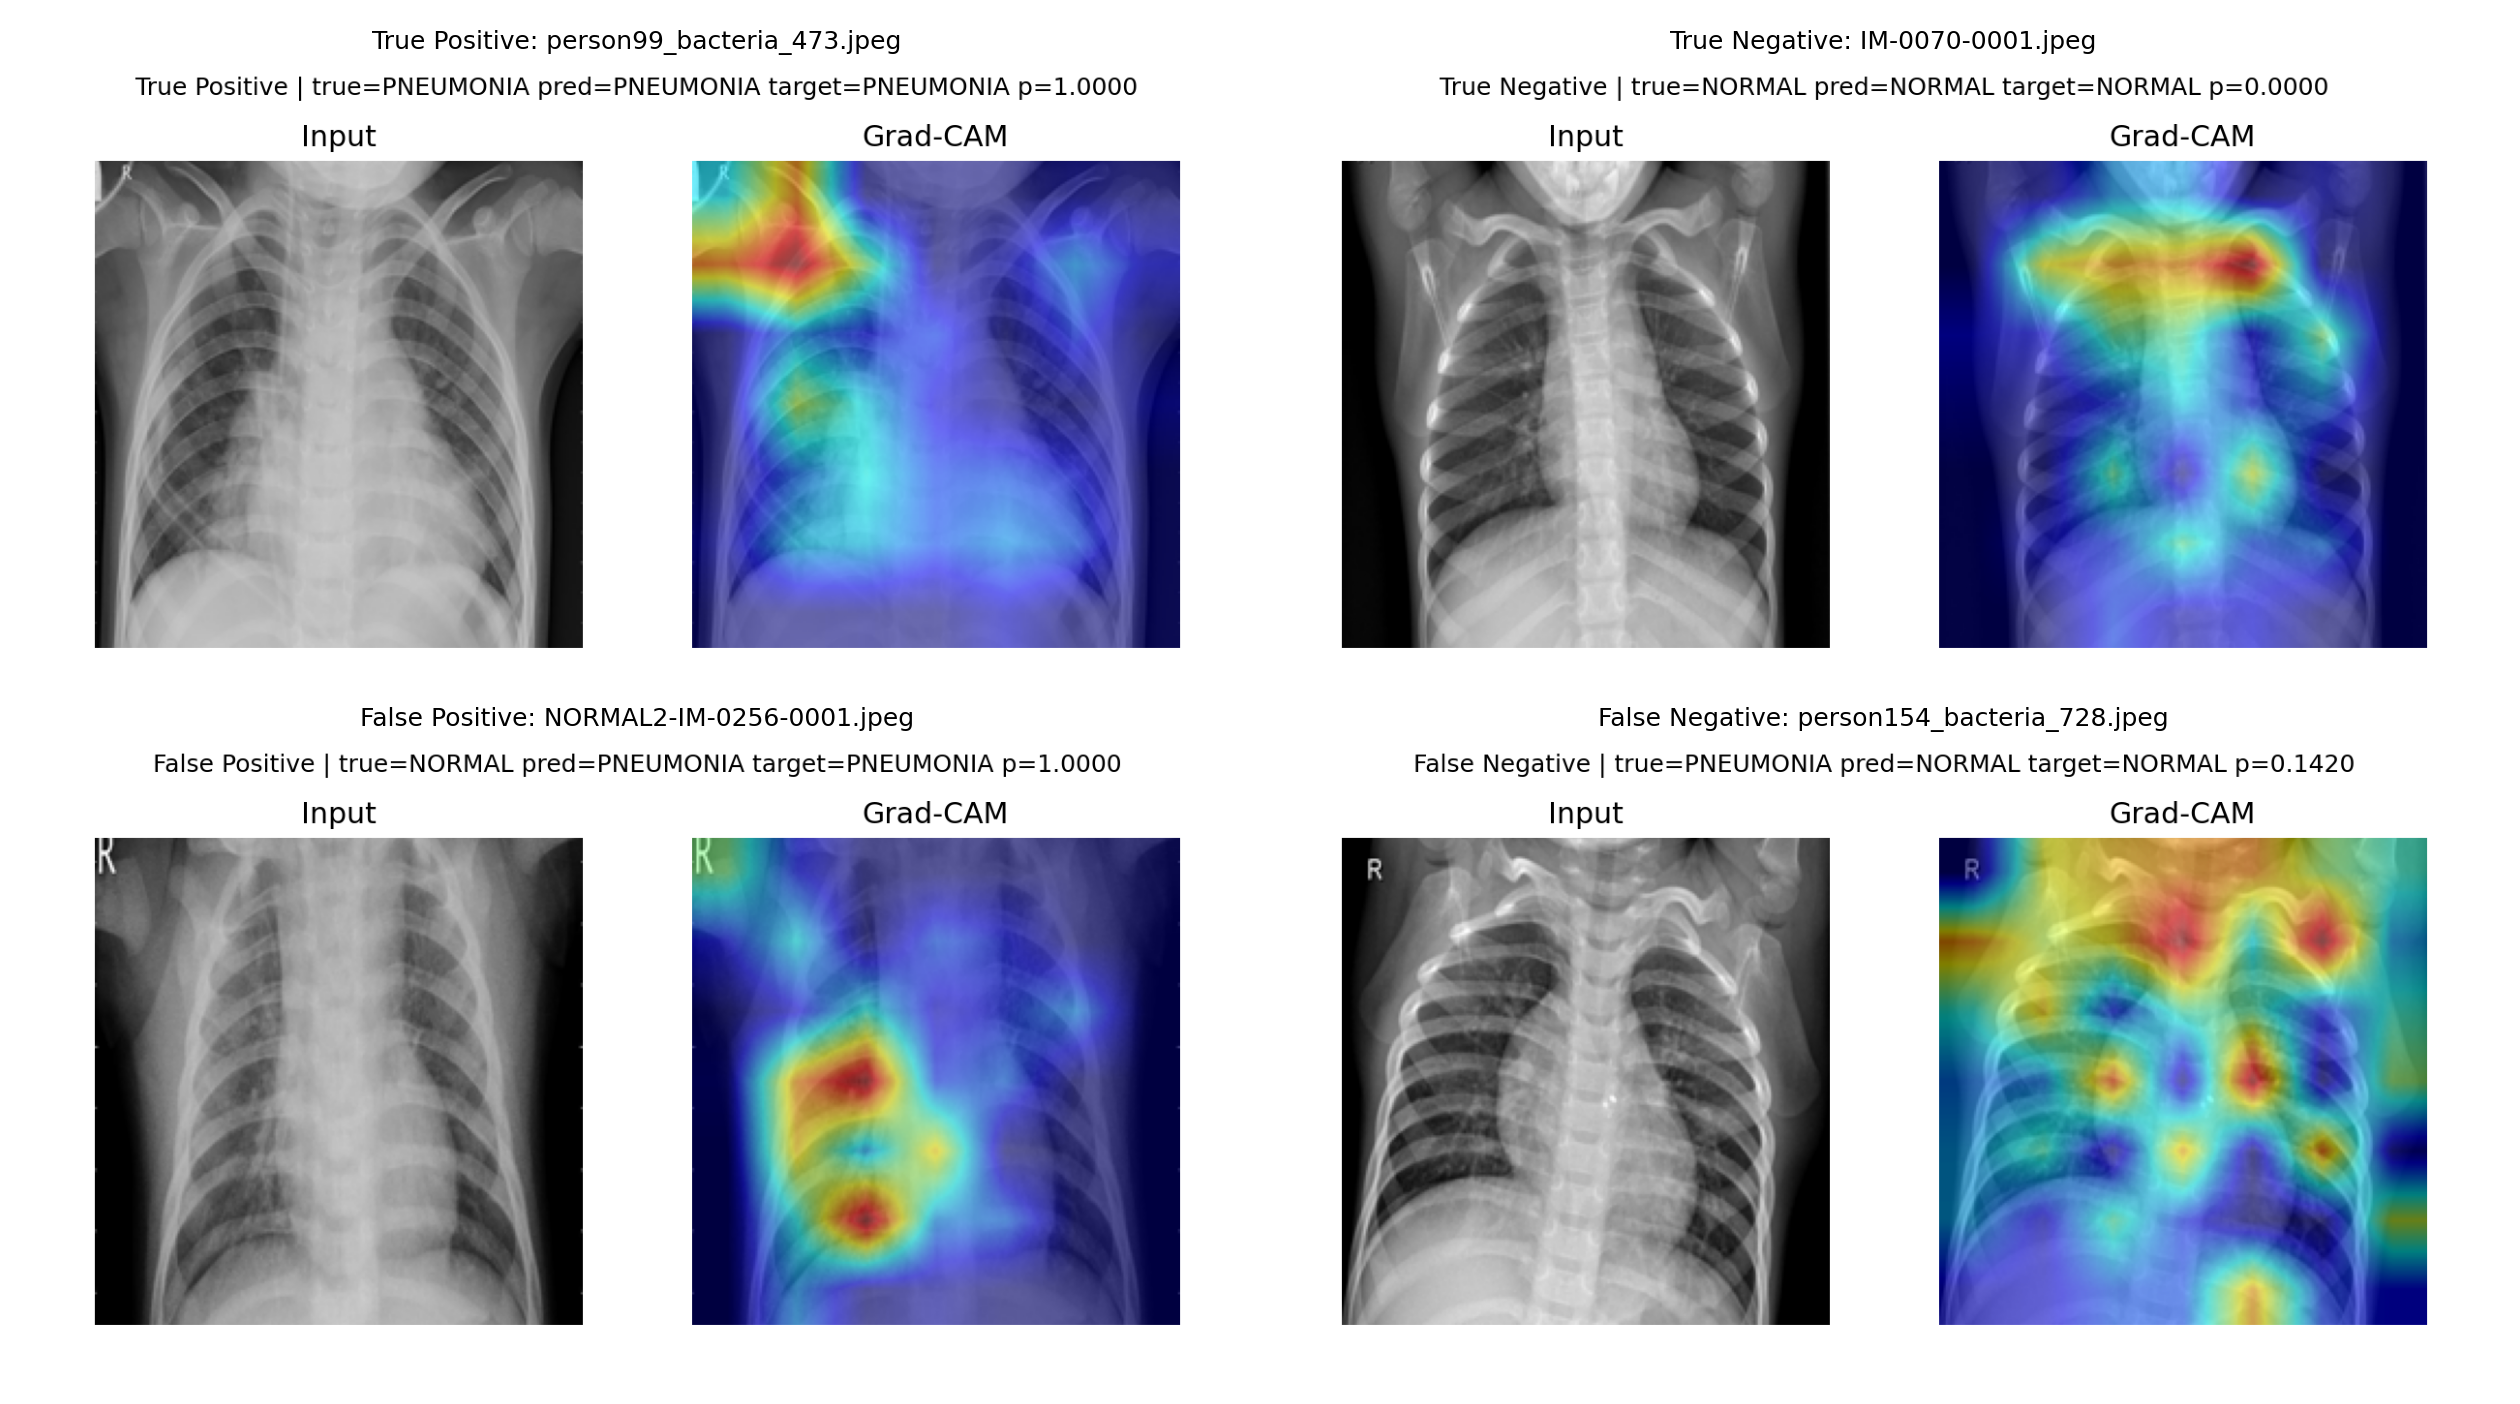
\includegraphics{../figures/grad_cam_examples_effnetv2.png}
\caption{EfficientNetV2-S 测试样本 Grad-CAM 可视化}
\end{figure}

部分 true positive
样本的热区覆盖胸腔内部较大区域，说明模型使用了与胸部结构相关的信息。部分
false positive
样本中，模型对正常图像给出了较高肺炎概率，热区有时集中在局部胸腔区域或图像边缘，这与正常样本误报现象一致。false
negative
样本的热图解释的是模型为什么倾向于正常类，不能解释为肺炎病灶位置。

Grad-CAM
可以帮助分析模型行为，但不能证明模型真正找到了医学病灶。本报告只将其作为定性解释材料，不作为临床证据。

\hypertarget{ux5355ux56feux4e0aux4f20ux7f51ux9875ux6f14ux793a}{%
\subsection{6
单图上传网页演示}\label{ux5355ux56feux4e0aux4f20ux7f51ux9875ux6f14ux793a}}

完成模型训练和测试后，课程设计制作了一个本地网页演示。这个页面不重新训练模型，只把已选定的
ViT-B/16 用于单张胸片推理。用户上传一张 X
光图片后，页面显示正常类概率、肺炎类概率和分类倾向。

网页由前端页面和本地推理服务组成。前端负责图片选择、影像预览和结果展示；后端读取上传图片，执行与测试阶段一致的预处理，再调用已训练的
ViT-B/16
做前向推理。用户选择图片后，页面先显示影像预览；点击分类按钮后，图片被发送到本地服务；后端将图片转换为三通道格式，统一缩放到
224 × 224，并按 ImageNet
均值和标准差归一化；模型输出正常类和肺炎类分数，经 softmax
转换为概率。演示页面使用默认阈值
0.5，当肺炎概率不低于该阈值时显示为疑似肺炎，否则显示为未见肺炎模式。

下图展示了网页的两种输出状态。左侧为正常样本，模型输出正常概率为
90.7\%，肺炎概率为
9.3\%，页面显示为未见肺炎模式；右侧为肺炎样本，模型输出肺炎概率为
99.5\%，页面显示为疑似肺炎。两张图说明网页可以完成单图上传、影像预览、概率输出和分类提示。该结果只代表模型在示例样本上的分类倾向，不能解释为真实临床诊断结论。

\begin{figure}
\centering
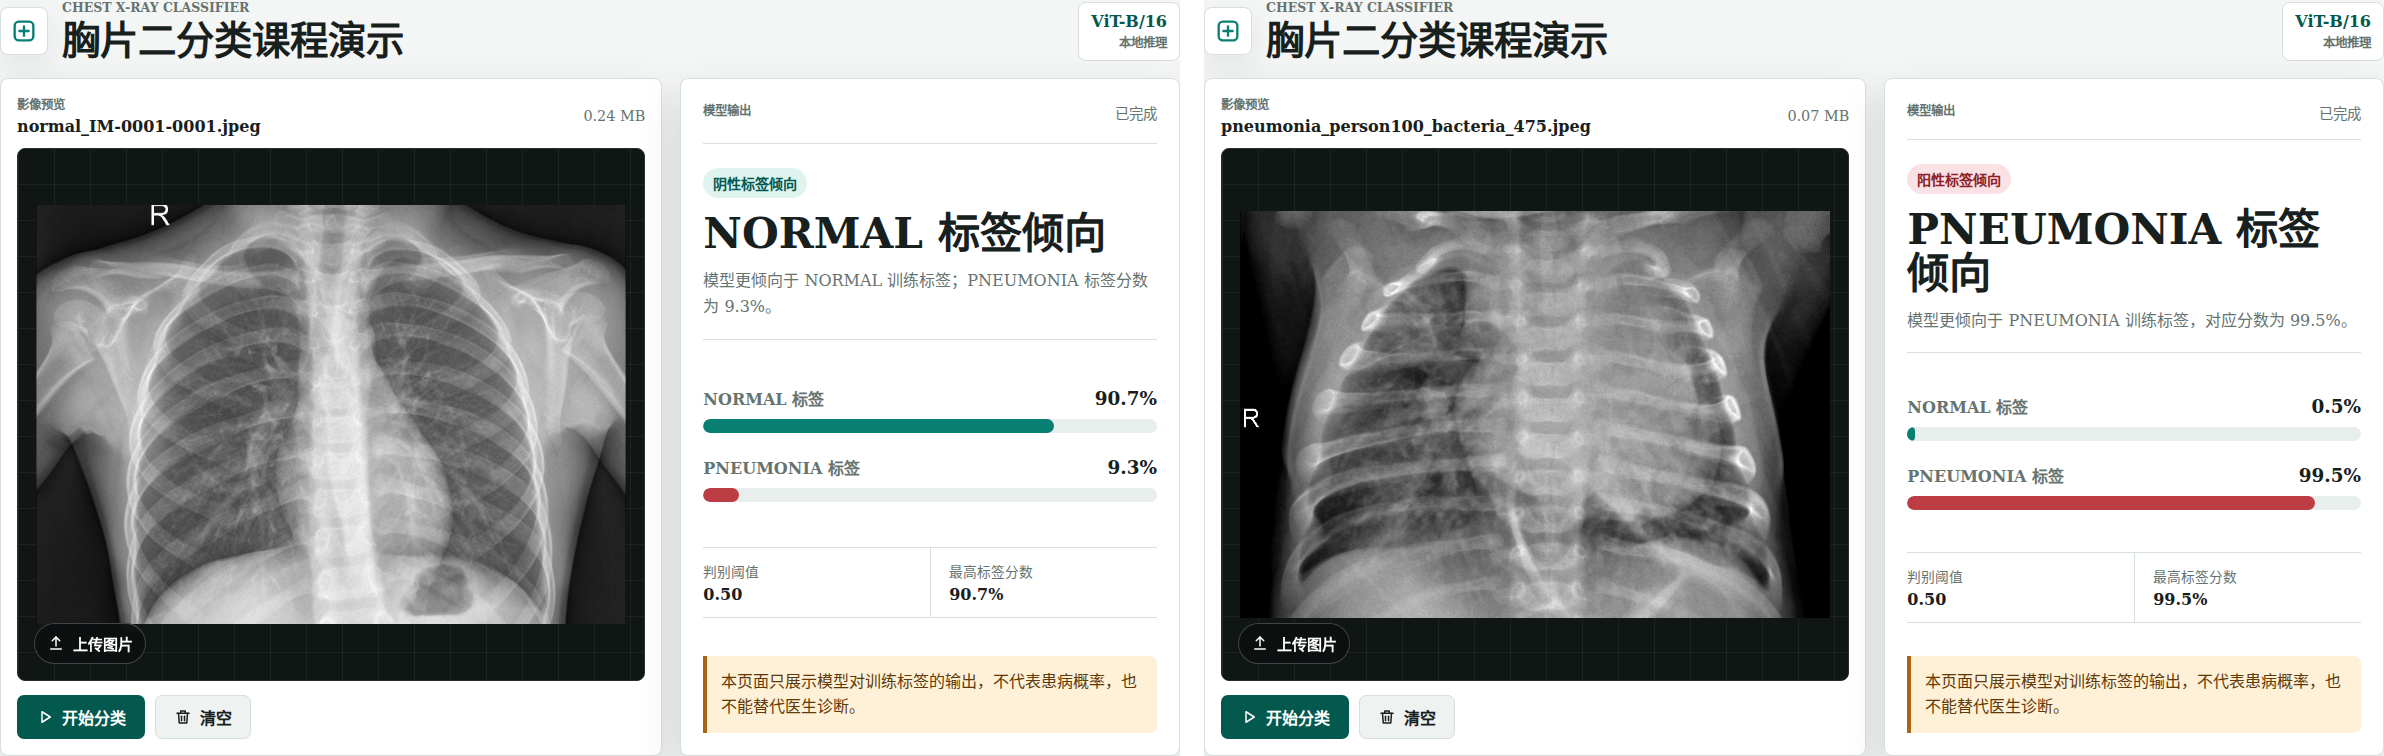
\includegraphics[width=1\textwidth,height=\textheight]{../figures/web_demo_examples.png}
\caption{单图上传网页正负样本并排展示}
\end{figure}

网页演示保留了课程设计结果的边界：不重新选择阈值，不使用测试集信息修改模型，也不把输出包装成医疗诊断。页面中提示结果仅用于课程设计演示；若实际存在症状或检查异常，应咨询专业医生。这样可以展示模型推理过程，也避免夸大实验模型的能力。

\hypertarget{ux8ba8ux8bba}{%
\subsection{7 讨论}\label{ux8ba8ux8bba}}

实验结果显示，预训练对该任务影响很明显。随机初始化 ViT-Small 的默认 F1
为 0.8469，预训练 ViT-B/16 的默认 F1 为 0.9248。对于 5856
张规模的胸片数据，直接从零训练 Transformer
并不占优，利用自然图像预训练权重进行迁移学习更合适。这也与 ViT
原始工作中``预训练后迁移到下游图像识别任务''的思路一致 {[}6{]}。

默认阈值和阈值扫描回答的是两个问题。默认阈值表现代表模型在不额外调阈值时的直接表现；阈值扫描反映模型分数在特定测试集上的可调节空间。在本组实验中，ViT-B/16
的默认阈值结果最好，EfficientNetV2-S 则在测试集阈值扫描后取得最高
F1。AUC
较高也不能自动等同于固定阈值表现最好，因为最终分类仍取决于阈值选择以及误报、漏检之间的取舍。

误差分析也说明，模型表现不能只用 F1 概括。ViT-B/16
加权模型是默认阈值下的主结果，但仍有 53
张正常图像被误报为肺炎，其中一部分还是高置信误报。对课程设计而言，这已经能说明模型具备一定的二分类能力；对真实医学场景而言，模型输出仍需要人工复核，高置信概率不能直接等同于诊断事实。

当前实验有几个限制。第一，验证集只有 16
张图像，不能承担稳定的模型选择或阈值校准功能。第二，训练集和测试集的类别比例并不完全一致，训练集肺炎比例更高，可能影响模型对肺炎类别的倾向。第三，测试集阈值扫描存在信息泄漏风险，只能作为分析，不能写成最终部署策略。第四，数据集中没有病灶级标注，Grad-CAM
热区不能解释为准确病灶定位。

为避免直接使用测试集选择阈值，实验尝试从训练集中划出独立校准集来选择
ViT-B/16
阈值。结果显示，校准集上的高分没有转化为官方测试集提升。现有结果足以支撑课程设计中的模型比较，但不足以支撑``已经获得稳定部署阈值''的说法。若继续改进，更应引入可靠的验证/校准数据，或做多次随机划分稳定性实验；继续在同一个测试集上寻找更高的阈值扫描分数意义有限。

\hypertarget{ux7ed3ux8bba}{%
\subsection{8 结论}\label{ux7ed3ux8bba}}

本课程设计完成了肺炎 X
光图像二分类实验。数据集完整性检查显示，本地共包含 5856
张有效胸片。EfficientNetV2-S 和 ViT-B/16
两条路线均能完成从图像输入到正常/肺炎概率输出的分类任务。

在默认 0.5 阈值下，预训练 ViT-B/16
加类别权重取得本组实验中最好的综合结果：accuracy 0.9006，precision
0.8779，recall 0.9769，specificity 0.7735，F1 0.9248，ROC-AUC
0.9710。相比 EfficientNetV2-S
无类别权重实验，它明显减少正常样本误报，并保持较高肺炎召回率。

在测试集阈值扫描中，原始 EfficientNetV2-S 取得最高 F1
0.9527，说明其分数排序能力仍然较强。由于该阈值来自测试集扫描，不能被表述为实际使用阈值。综合默认阈值和误差结构，预训练
ViT-B/16 更适合作为本报告的主模型，EfficientNetV2-S
的扫描结果保留为阈值权衡分析。

独立校准集实验没有提升官方测试集结果，因此报告保留 ViT-B/16
默认阈值作为主模型结论，并明确阈值校准受数据划分限制。该结果可以满足课程设计对实验流程、模型比较和误差分析的要求，但不能扩展为临床部署结论。

应用展示部分实现了本地网页演示，支持单张 X
光图片上传、影像预览、模型推理和概率展示。网页只用于课程设计展示，不用于临床诊断。

\hypertarget{ux53c2ux8003ux6587ux732e}{%
\subsection{参考文献}\label{ux53c2ux8003ux6587ux732e}}

\begin{enumerate}
\def\labelenumi{\arabic{enumi}.}
\tightlist
\item
  Kermany D, Zhang K, Goldbaum M. Labeled Optical Coherence Tomography
  (OCT) and Chest X-Ray Images for Classification. Mendeley Data, V2,
  2018. DOI: 10.17632/rscbjbr9sj.2.
\item
  Kermany D S, Goldbaum M, Cai W, et al.~Identifying Medical Diagnoses
  and Treatable Diseases by Image-Based Deep Learning. Cell, 2018,
  172(5): 1122-1131.e9. DOI: 10.1016/j.cell.2018.02.010.
\item
  Litjens G, Kooi T, Bejnordi B E, et al.~A survey on deep learning in
  medical image analysis. Medical Image Analysis, 2017, 42: 60-88. DOI:
  10.1016/j.media.2017.07.005.
\item
  Rajpurkar P, Irvin J, Zhu K, et al.~CheXNet: Radiologist-level
  pneumonia detection on chest X-rays with deep learning.
  arXiv:1711.05225, 2017. DOI: 10.48550/arXiv.1711.05225.
\item
  Tan M, Le Q V. EfficientNetV2: Smaller Models and Faster Training.
  Proceedings of the 38th International Conference on Machine Learning,
  2021: 10096-10106.
\item
  Dosovitskiy A, Beyer L, Kolesnikov A, et al.~An Image is Worth 16x16
  Words: Transformers for Image Recognition at Scale. ICLR, 2021.
\item
  Selvaraju R R, Cogswell M, Das A, et al.~Grad-CAM: Visual Explanations
  from Deep Networks via Gradient-Based Localization. ICCV, 2017:
  618-626. DOI: 10.1109/ICCV.2017.74.
\item
  Singh S, Kumar M, Kumar A, et al.~Efficient pneumonia detection using
  Vision Transformers on chest X-rays. Scientific Reports, 2024, 14:
  2487. DOI: 10.1038/s41598-024-52703-2.
\end{enumerate}

\hypertarget{ux9644ux5f55ux9879ux76eeux63d0ux5347ux7248ux8865ux5145ux5b9eux9a8c}{%
\clearpage
\subsection{9 跨数据集泛化、校准与错误分析}\label{sec:generalization}}

\hypertarget{a.1-ux5f53ux524dux57faux7ebfux51bbux7ed3}{%
\subsubsection{9.1
当前基线冻结}\label{a.1-ux5f53ux524dux57faux7ebfux51bbux7ed3}}

提升版实验不覆盖原有 Kermany 主结果。ViT-B/16 默认阈值 0.5
仍作为主模型结果，checkpoint 的 SHA256 为
\texttt{78604698f504d8d96f5bdad9570608c77472e7625684cb13a6f222275c8381be}。基线清单保存在
\texttt{results/baseline\_manifest.json}。该清单记录测试集样本数、混淆矩阵、主指标和受保护输出文件。

\hypertarget{a.2-ux65b0ux589eux6a21ux578bux5bf9ux7167}{%
\subsubsection{9.2
新增模型对照}\label{a.2-ux65b0ux589eux6a21ux578bux5bf9ux7167}}

提升计划建议加入 DenseNet121 和 ConvNeXt-Tiny。本轮已补齐两个 ImageNet
预训练模型的 Kermany test 评价。结果显示，DenseNet121 默认阈值 F1 略高于
ViT-B/16，ConvNeXt-Tiny 的 AUC 最高，但默认阈值 F1 低于 DenseNet121 和
ViT-B/16。

\begin{longtable}[]{@{}
  >{\raggedright\arraybackslash}p{(\columnwidth - 14\tabcolsep) * \real{0.1000}}
  >{\raggedright\arraybackslash}p{(\columnwidth - 14\tabcolsep) * \real{0.1000}}
  >{\raggedleft\arraybackslash}p{(\columnwidth - 14\tabcolsep) * \real{0.1333}}
  >{\raggedleft\arraybackslash}p{(\columnwidth - 14\tabcolsep) * \real{0.1333}}
  >{\raggedleft\arraybackslash}p{(\columnwidth - 14\tabcolsep) * \real{0.1333}}
  >{\raggedleft\arraybackslash}p{(\columnwidth - 14\tabcolsep) * \real{0.1333}}
  >{\raggedleft\arraybackslash}p{(\columnwidth - 14\tabcolsep) * \real{0.1333}}
  >{\raggedleft\arraybackslash}p{(\columnwidth - 14\tabcolsep) * \real{0.1333}}@{}}
\toprule\noalign{}
\begin{minipage}[b]{\linewidth}\raggedright
模型
\end{minipage} & \begin{minipage}[b]{\linewidth}\raggedright
预训练
\end{minipage} & \begin{minipage}[b]{\linewidth}\raggedleft
Acc
\end{minipage} & \begin{minipage}[b]{\linewidth}\raggedleft
Prec
\end{minipage} & \begin{minipage}[b]{\linewidth}\raggedleft
Rec
\end{minipage} & \begin{minipage}[b]{\linewidth}\raggedleft
Spec
\end{minipage} & \begin{minipage}[b]{\linewidth}\raggedleft
F1
\end{minipage} & \begin{minipage}[b]{\linewidth}\raggedleft
AUC
\end{minipage} \\
\midrule\noalign{}
\endhead
\bottomrule\noalign{}
\endlastfoot
ViT-B/16 & ImageNet & 0.9006 & 0.8779 & 0.9769 & 0.7735 & 0.9248 &
0.9710 \\
DenseNet121 & ImageNet & 0.9054 & 0.8770 & 0.9872 & 0.7692 & 0.9288 &
0.9743 \\
ConvNeXt-Tiny & ImageNet & 0.8878 & 0.8524 & 0.9923 & 0.7137 & 0.9171 &
0.9781 \\
\end{longtable}

DenseNet121 的误报为 54 张、漏检为 5 张。ConvNeXt-Tiny 的误报为 67
张、漏检为 3 张。DenseNet121 在默认阈值下略优于
ViT-B/16，但二者差距很小；ConvNeXt-Tiny
的排序能力较强，但默认阈值下正常误报更多。

\hypertarget{a.3-ux6982ux7387ux6821ux51c6ux4e0eux53efux9760ux6027}{%
\subsubsection{9.3
概率校准与可靠性}\label{a.3-ux6982ux7387ux6821ux51c6ux4e0eux53efux9760ux6027}}

ViT-B/16 在 Kermany test 上的未校准 ECE 为 0.0645，Brier score 为
0.0850。使用官方 val 的 16 张图像学习 temperature scaling 后，ECE 变为
0.0858，Brier score 变为 0.0918。这个结果说明 Kermany 官方 val
太小，不适合支撑稳定概率校准。

扩容 RSNA 后，val 包含 NORMAL 107 张和 PNEUMONIA 106
张，达到本轮提升计划的最低校准样本要求。Kermany 训练的 ViT-B/16 直接测试
RSNA test 时，未校准 ECE 为 0.1919，Brier score 为 0.2434；使用 RSNA val
学习温度参数后，temperature 为 4.27，RSNA test ECE 降到 0.0263，Brier
score 降到 0.2041。DenseNet121 的对应结果为：未校准 ECE 0.1968、Brier
score 0.2325；temperature 为 4.14，校准后 ECE 0.0272、Brier score
0.1874。

\begin{longtable}[]{@{}
  >{\raggedright\arraybackslash}p{(\columnwidth - 10\tabcolsep) * \real{0.1429}}
  >{\raggedright\arraybackslash}p{(\columnwidth - 10\tabcolsep) * \real{0.1429}}
  >{\raggedright\arraybackslash}p{(\columnwidth - 10\tabcolsep) * \real{0.1429}}
  >{\raggedleft\arraybackslash}p{(\columnwidth - 10\tabcolsep) * \real{0.1905}}
  >{\raggedleft\arraybackslash}p{(\columnwidth - 10\tabcolsep) * \real{0.1905}}
  >{\raggedleft\arraybackslash}p{(\columnwidth - 10\tabcolsep) * \real{0.1905}}@{}}
\toprule\noalign{}
\begin{minipage}[b]{\linewidth}\raggedright
模型
\end{minipage} & \begin{minipage}[b]{\linewidth}\raggedright
测试集
\end{minipage} & \begin{minipage}[b]{\linewidth}\raggedright
校准方式
\end{minipage} & \begin{minipage}[b]{\linewidth}\raggedleft
Temperature
\end{minipage} & \begin{minipage}[b]{\linewidth}\raggedleft
ECE
\end{minipage} & \begin{minipage}[b]{\linewidth}\raggedleft
Brier
\end{minipage} \\
\midrule\noalign{}
\endhead
\bottomrule\noalign{}
\endlastfoot
ViT-B/16 & Kermany & 未校准 & - & 0.0645 & 0.0850 \\
ViT-B/16 & Kermany & 官方 val temperature scaling & 0.50 & 0.0858 &
0.0918 \\
ViT-B/16 & RSNA & 未校准 & - & 0.1919 & 0.2434 \\
ViT-B/16 & RSNA & RSNA val temperature scaling & 4.27 & 0.0263 &
0.2041 \\
DenseNet121 & RSNA & 未校准 & - & 0.1968 & 0.2325 \\
DenseNet121 & RSNA & RSNA val temperature scaling & 4.14 & 0.0272 &
0.1874 \\
\end{longtable}

校准改善的是概率可信度，不等于分类能力被直接提高。报告中应把 ECE、Brier
与 accuracy、recall、specificity 分开解释。

\hypertarget{a.4-ux9519ux8befux6837ux672cux5206ux6790}{%
\subsubsection{9.4
错误样本分析}\label{a.4-ux9519ux8befux6837ux672cux5206ux6790}}

错误样本分析脚本导出了 false positive、false
negative、高置信错误和边界样本。Kermany test 上，ViT-B/16 在默认阈值下有
53 个 false positive、9 个 false negative、11 个 0.4 到 0.6
区间的边界样本。其中高置信 false positive 为 33 个，高置信 false
negative 为 2
个。这说明主数据集上的主要错误来自正常样本被模型高置信推向肺炎类。

扩容 RSNA test 上，Kermany 训练的 ViT-B/16 有 106 个 false positive、30
个 false negative 和 30 个边界样本；Kermany 训练的 DenseNet121 有 97 个
false positive、21 个 false negative 和 18
个边界样本。两者都以正常样本误报为主，与外部测试 specificity 偏低一致。

DenseNet121 作为新增 CNN 强基线，已生成 Kermany 错误样本 Grad-CAM、扩容
RSNA 外部 true positive Grad-CAM 和 NIH 外部 true positive
Grad-CAM。热图只说明模型分类贡献区域，不能写成病灶定位。

对应文件：

\begin{Shaded}
\begin{Highlighting}[]
\NormalTok{results/error\_cases\_kermany\_test\_vit\_b16.csv}
\NormalTok{results/error\_summary\_kermany\_test\_vit\_b16.json}
\NormalTok{figures/error\_case\_grid\_kermany\_test\_vit\_b16.png}
\NormalTok{figures/reliability\_kermany\_test\_vit\_b16\_uncalibrated.png}
\NormalTok{figures/gradcam\_kermany\_error\_cases\_densenet121.png}
\NormalTok{figures/gradcam\_rsna\_positive\_cases\_densenet121\_expanded.png}
\NormalTok{figures/gradcam\_nih\_positive\_cases\_densenet121.png}
\end{Highlighting}
\end{Shaded}

\hypertarget{a.5-ux5916ux90e8ux9a8cux8bc1ux72b6ux6001}{%
\subsubsection{9.5
外部验证状态}\label{a.5-ux5916ux90e8ux9a8cux8bc1ux72b6ux6001}}

RSNA 数据处理、检查、固定划分和 manifest 生成脚本已经补齐。本轮使用
Hugging Face 镜像 \texttt{Baldezo313/rsna-pneumonia-dataset} 扩容得到
1707 张二分类图像，train 为 NORMAL 560 / PNEUMONIA 492，val 为 107 /
106，test 为 215 / 227。test 每类已经超过 200
张，达到本提升计划设定的最低外部验证门槛。

Kermany 训练模型直接迁移到扩容 RSNA test 后，ViT-B/16 F1 为
0.7434、DenseNet121 F1 为 0.7774、ConvNeXt-Tiny F1 为
0.7556。DenseNet121 仍相对最好，但 accuracy 只有 0.7330，specificity
只有 0.5488，说明主要问题仍是正常样本误报。该结果比 88 张 pilot
更有说服力，也更清楚地支持``单数据集高分不能代表跨来源稳定性''。

扩容后补充了 DenseNet121 的
RSNA-only、简单混合、domain-balanced、冻结分类头和最后 block
解冻。简单混合训练在 RSNA test 上 accuracy 为 0.7602、specificity 为
0.8837，但 recall 降到 0.6432，且 Kermany test accuracy 降到
0.8606。domain-balanced 在 Kermany test 上保持 accuracy 0.9022、F1
0.9266，但 RSNA test F1 为 0.7098。冻结分类头和最后 block 解冻在 RSNA
test 上分别取得 F1 0.7812 和 0.7826，但 specificity 仍只有 0.6047 和
0.5581。也就是说，训练策略可以改变误报/漏检权衡，但没有出现同时稳定提升
Kermany 与 RSNA 的简单方案。

NIH ChestX-ray14 的 \texttt{Pneumonia} vs \texttt{No\ Finding}
弱标签子集作为第二个压力测试。该子集来自 \texttt{images\_001.zip}，共
130 张图像，其中 train 92 张、val 12 张、test 26 张。Kermany
训练模型直接迁移到 NIH test 后表现也明显下降：ViT-B/16 F1 为
0.4800，DenseNet121 F1 为 0.5385，ConvNeXt-Tiny F1 为 0.5000。RSNA
已经从小样本 pilot 扩到最低外部验证规模，但仍不是全量挑战数据；NIH
标签来自报告文本挖掘。因此这些结果可以支持跨来源风险分析，不能写成稳定临床外部验证。

全模型低学习率微调作为最后一组适配对照，从同一个 Kermany DenseNet121
checkpoint 出发，在 RSNA train 上训练三个 epoch。该策略在 RSNA test 上得到
accuracy 0.7217、recall 0.9295、specificity 0.5023、F1 0.7743 和 AUC
0.8343；回测 Kermany test 时 accuracy 为 0.8766、F1 为 0.9087。它保持了较高
召回率，但没有同时保住两个数据集上的综合性能。完整策略矩阵说明，适配方式主要改变
误报与漏检的权衡，目前没有一种简单策略能在两个来源上同步改善。

\clearpage
\subsection{10 系统实现与复现设计}

网页演示、训练、评价、校准和错误分析共享相同的类别顺序、图像缩放和 ImageNet
归一化规则。网页只加载冻结的主模型权重，不会在上传样本后更新模型参数。输出包括
两类概率和阈值为 0.5 的分类提示，页面文字明确限制在课程展示场景。

复现实验时，先检查数据目录和图像可读性，再按照固定 seed=42 生成 RSNA 划分。
外部测试、校准和训练策略都使用同一份 test 清单。温度参数只从 validation split
学习；测试集只用于评价。每次训练输出独立摘要和 checkpoint 路径，新增实验不会覆盖
冻结的 Kermany 主结果。汇总表保留全部策略，而非只选择最好的一行。

主结果可追溯到预测 CSV 和评价 JSON。数据规模可追溯到 dataset summary；温度缩放
可追溯到 calibration JSON；错误类型可追溯到 error cases CSV；报告图表来自这些
结构化文件。图表不承担独立结论，正文中的数值判断同时给出数据集、split 和模型来源。

\clearpage
\subsection{11 讨论与限制}

Kermany test 上三个预训练模型的 F1 均超过 0.91，但在 RSNA test 上下降到
0.74--0.78。这个差异比单个模型之间的结构差异更大，说明数据来源变化是当前项目的
主要风险。RSNA 图像来自不同人群和采集流程，标签定义也与 Kermany 文件夹标签不同，
因此不能把两个测试集上的数值当成同一难度下的直接排名。

RSNA 扩容解决了几十张样本造成的明显不稳定问题，但本项目只使用镜像中可获得的
1707 张图像，并非完整挑战数据。NIH 只有 130 张弱标签图像，其中肺炎标签来自报告
文本挖掘，不能与人工精标数据等同。Kermany 原始 validation split 只有 16 张，导致
主数据集温度缩放反而变差；这个负结果反映校准样本不足。

训练策略比较使用固定 seed=42，没有多随机种子置信区间。因此，本报告可以讨论当前
固定划分上的误报、漏检和域偏移现象，但不能宣称某个策略具有统计意义上的稳定优势。
Grad-CAM 没有经过定位指标验证，只用于观察分类贡献区域，不能称为病灶定位。

本项目仅使用去标识化公开数据，不收集新的患者信息。网页演示在本地运行，不上传图像
到第三方服务。模型不具备临床验证、风险管理或真实医疗工作流评估，不能用于患者诊断
或治疗决策。

\clearpage
\subsection{12 结论}

本课程设计完成了从数据检查、迁移学习训练、主数据集评价到跨数据集泛化分析的完整
实验链。Kermany test 上 DenseNet121 默认阈值 F1 为 0.9288。扩容 RSNA test
达到每类至少 200 张后，三个模型的 specificity 和 F1 均明显下降，主要错误是正常
样本被判为肺炎。

RSNA val 温度缩放明显降低 ECE 和 Brier score，但不改变阈值为 0.5 时的分类排序
能力。RSNA-only、简单混合、域均衡、冻结分类头、最后 block 解冻和全模型低学习率
微调均已比较。不同策略能调整 sensitivity--specificity 权衡，却没有找到同时稳定
提高 Kermany 与 RSNA 综合指标的简单方案。

项目支持的结论限于：单一公开数据集上的高分不能代表跨来源稳定性；评价胸片二分类
模型时需要同时观察外部测试、概率校准和错误结构。它不支持临床可用性、病灶定位能力
或替代医生的判断。

\clearpage
\appendix
\subsection{附录 A：关键图表与逐图解释}

本附录集中呈现报告结论所依赖的图像证据。每张图均对应结构化预测或评价结果，用于
核对正文中的误报、漏检、域偏移、校准和适配策略判断。

\newcommand{\evidencefigure}[3]{\clearpage\subsubsection{#1}\begin{center}
\includegraphics[width=0.90\textwidth,height=0.72\textheight,keepaspectratio]{#2}
\end{center}#3}

\evidencefigure{A.1 Kermany 主模型混淆矩阵}{../figures/confusion_matrix_test_reproduced_vit_b16.png}{主要剩余错误是正常样本误报，漏检数量较少。}
\evidencefigure{A.2 DenseNet121 主数据集混淆矩阵}{../figures/confusion_matrix_kermany_test_densenet121.png}{DenseNet121 保持高召回，但正常类特异性仍低于 0.8。}
\evidencefigure{A.3 ConvNeXt-Tiny 主数据集混淆矩阵}{../figures/confusion_matrix_kermany_test_convnext_tiny.png}{ConvNeXt-Tiny 漏检少，但误报高于另外两个预训练模型。}
\evidencefigure{A.4 RSNA ViT-B/16 混淆矩阵}{../figures/confusion_matrix_rsna_test_vit_b16.png}{正常类误报明显增加，反映阈值和特征分布迁移。}
\evidencefigure{A.5 RSNA DenseNet121 混淆矩阵}{../figures/confusion_matrix_rsna_test_densenet121.png}{直接迁移综合表现相对较好，但 specificity 仍只有 0.5488。}
\evidencefigure{A.6 RSNA ConvNeXt-Tiny 混淆矩阵}{../figures/confusion_matrix_rsna_test_convnext_tiny.png}{模型保持高 recall，同时产生大量正常样本误报。}
\evidencefigure{A.7 RSNA-only 训练}{../figures/confusion_matrix_rsna_test_densenet121_expanded_rsna_only.png}{RSNA-only 提高正常类识别，但回测 Kermany 时跨域损失明显。}
\evidencefigure{A.8 简单混合训练}{../figures/confusion_matrix_rsna_test_densenet121_expanded_simple_mixed.png}{简单混合提高 specificity，却使 recall 降到 0.6432。}
\evidencefigure{A.9 域均衡训练}{../figures/confusion_matrix_rsna_test_densenet121_expanded_domain_balanced.png}{域均衡更好地保存 Kermany 性能，但没有提高 RSNA F1。}
\evidencefigure{A.10 冻结分类头适配}{../figures/confusion_matrix_rsna_test_densenet121_expanded_finetune_head.png}{只训练分类头保持较高 recall，正常误报仍较多。}
\evidencefigure{A.11 最后特征块解冻}{../figures/confusion_matrix_rsna_test_densenet121_expanded_last_block.png}{增加可训练层后 recall 升高，但 specificity 未改善。}
\evidencefigure{A.12 全模型低学习率微调}{../figures/confusion_matrix_rsna_test_densenet121_expanded_full_finetune.png}{完整微调没有超过直接迁移，Kermany 性能同时下降。}
\evidencefigure{A.13 Kermany ViT 概率分布}{../figures/probability_distribution_test_vit_b16.png}{两类概率总体可分，但正常类存在高肺炎概率长尾。}
\evidencefigure{A.14 RSNA ViT 概率分布}{../figures/probability_distribution_rsna_test_vit_b16.png}{外部数据两类概率重叠增大，与较低 specificity 一致。}
\evidencefigure{A.15 RSNA DenseNet 概率分布}{../figures/probability_distribution_rsna_test_densenet121.png}{正常样本高分尾部仍是主要误报来源。}
\evidencefigure{A.16 主模型阈值曲线}{../figures/threshold_curve_test_reproduced_vit_b16.png}{测试集阈值扫描只展示权衡，不能作为无偏部署阈值。}
\evidencefigure{A.17 Kermany ViT 可靠性}{../figures/reliability_kermany_test_vit_b16_uncalibrated.png}{主数据集概率仍存在一定过度自信。}
\evidencefigure{A.18 RSNA ViT 可靠性}{../figures/reliability_rsna_test_vit_b16.png}{温度缩放后 ECE 降低，但混淆矩阵不因此改变。}
\evidencefigure{A.19 RSNA DenseNet 可靠性}{../figures/reliability_rsna_test_densenet121.png}{外部校准改善概率可信度，不代表准确率提高。}
\evidencefigure{A.20 Kermany ViT 错误样本}{../figures/error_case_grid_kermany_test_vit_b16.png}{高置信误报说明错误不只集中在阈值附近。}
\evidencefigure{A.21 Kermany DenseNet 错误样本}{../figures/error_case_grid_kermany_test_densenet121.png}{主要错误结构同样以正常误报为主。}
\evidencefigure{A.22 RSNA ViT 错误样本}{../figures/error_case_grid_rsna_test_vit_b16.png}{外部错误图像在亮度、裁剪和纹理上存在差异。}
\evidencefigure{A.23 RSNA DenseNet 错误样本}{../figures/error_case_grid_rsna_test_densenet121.png}{错误网格用于检查失败类型，不用于医学诊断。}
\evidencefigure{A.24 全模型微调错误样本}{../figures/error_case_grid_rsna_test_densenet121_expanded_full_finetune.png}{完整微调后仍保留大量正常误报。}
\evidencefigure{A.25 Kermany DenseNet Grad-CAM}{../figures/gradcam_kermany_error_cases_densenet121.png}{热图展示分类贡献区域，不证明真实病灶位置。}
\evidencefigure{A.26 RSNA DenseNet Grad-CAM}{../figures/gradcam_rsna_positive_cases_densenet121_expanded.png}{跨来源关注区域差异只作定性观察。}
\evidencefigure{A.27 NIH DenseNet Grad-CAM}{../figures/gradcam_nih_positive_cases_densenet121.png}{弱标签热图不具备定位真值。}
\evidencefigure{A.28 RSNA 类别分布}{../figures/rsna_class_distribution.png}{固定划分满足 test 每类超过 200 张。}
\evidencefigure{A.29 NIH 类别分布}{../figures/nih_class_distribution.png}{NIH 规模很小，只承担弱标签补充压力测试。}
\evidencefigure{A.30 网页演示}{../figures/web_demo_examples.png}{网页展示单图概率输出，不代表临床系统。}

\clearpage
\subsection{附录 B：复现验收表}

\begin{longtable}[]{@{}p{0.22\textwidth}p{0.30\textwidth}p{0.38\textwidth}@{}}
\toprule
验收对象 & 核对方法 & 通过标准 \\
\midrule
Kermany 基线 & 核对冻结清单、权重哈希和复现评价 & 混淆矩阵为 181/53/9/381，主结果未被覆盖 \\
RSNA 数据 & 核对固定划分和数据检查报告 & train、val、test 均含两类，test 每类不少于 200 \\
模型比较 & 核对三种预训练模型的双数据集结果 & 指标包含 accuracy、recall、specificity、F1 和 AUC \\
策略矩阵 & 核对六种 DenseNet121 训练路线 & 每组同时保留 RSNA 与 Kermany 测试结果 \\
概率校准 & 核对温度来源和可靠性文件 & 温度只由 validation 学习，test 不参与拟合 \\
错误分析 & 核对错误 CSV、摘要和网格图 & FP、FN、高置信错误和边界样本可追溯 \\
可解释性 & 核对三来源 Grad-CAM & 图注不使用病灶定位或临床诊断表述 \\
软件测试 & 运行自动测试 & 全部测试通过 \\
报告 & 独立编译 LaTeX 并检查 PDF & 页数超过 50，图表可见，无致命编译错误 \\
\bottomrule
\end{longtable}

验收表只确认仓库中已经存在并能复查的证据。没有多随机种子统计、完整 RSNA 挑战
数据和临床验证，因此这些内容继续作为限制，不转化为完成声明。

\end{document}
